% !TeX program = xelatex
\documentclass[a4paper,10pt]{article}

% ============================================================================
% កញ្ចប់សម្ភារៈសិក្សាបោះពុម្ព ស-ខ្មៅ (Printable Classroom Materials - Grade 8 2.2 ISO)
% ត្រូវគ្នា ១០០% នឹង LS_Plan_ISO.tex និង Teaching_Scenario_ISO.tex
% ============================================================================
\usepackage[a4paper, left=1.0cm, right=1.0cm, top=0.75cm, bottom=1.05cm, footskip=0.55cm]{geometry}
\usepackage{amsmath, amssymb}
\usepackage{unicode-math}
\usepackage{fontspec}
\usepackage{array, colortbl}
\usepackage[table]{xcolor}
\usepackage{enumitem}
\usepackage{pifont}
\usepackage{fancyhdr}
\usepackage{lastpage}
\usepackage{tikz}
\usepackage[most]{tcolorbox}
\usetikzlibrary{calc, arrows.meta, angles, quotes, decorations.markings, positioning, babel}

% LaTeX 2025 compatibility guard
\makeatletter
\let\@expl@@@mark@update@singlecol@structures@@\relax
\makeatother

% ============================================================================
% ការកំណត់ពុម្ពអក្សរផ្លូវការ (Word-Styled Khmer + Cambria Math + Times New Roman)
% ============================================================================
% Cross-platform font path resolver (Windows local + Linux/Cloud repo fonts/)
\providecommand{\NGSFindFonts}{%
  \IfFileExists{C:/Windows/Fonts/cambria.ttc}{%
    \def\NGSSysPath{C:/Windows/Fonts/}%
    \def\NGSUserPath{C:/Users/KIT/AppData/Local/Microsoft/Windows/Fonts/}%
  }{%
    \IfFileExists{./fonts/KhmerOSsiemreap.ttf}{\def\NGSSysPath{./fonts/}\def\NGSUserPath{./fonts/}}{%
    \IfFileExists{../fonts/KhmerOSsiemreap.ttf}{\def\NGSSysPath{../fonts/}\def\NGSUserPath{../fonts/}}{%
    \IfFileExists{../../fonts/KhmerOSsiemreap.ttf}{\def\NGSSysPath{../../fonts/}\def\NGSUserPath{../../fonts/}}{%
    \IfFileExists{../../../fonts/KhmerOSsiemreap.ttf}{\def\NGSSysPath{../../../fonts/}\def\NGSUserPath{../../../fonts/}}{%
    \IfFileExists{../../../../fonts/KhmerOSsiemreap.ttf}{\def\NGSSysPath{../../../../fonts/}\def\NGSUserPath{../../../../fonts/}}{%
    \IfFileExists{../../../../../fonts/KhmerOSsiemreap.ttf}{\def\NGSSysPath{../../../../../fonts/}\def\NGSUserPath{../../../../../fonts/}}{%
    \IfFileExists{../../../../../../fonts/KhmerOSsiemreap.ttf}{\def\NGSSysPath{../../../../../../fonts/}\def\NGSUserPath{../../../../../../fonts/}}{%
      \def\NGSSysPath{../../../../../../../fonts/}\def\NGSUserPath{../../../../../../../fonts/}%
    }}}}}}}%
  }%
}
\NGSFindFonts

\setmathfont[
  Path={\NGSSysPath},
  FontIndex=1,
  Scale=1.02
]{cambria.ttc}

\defaultfontfeatures{Ligatures=TeX}

\setmainfont[
  Path={\NGSUserPath},
  Extension=.ttf,
  Script=Khmer,
  BoldFont={KhmerOSsiemreap},
  BoldFeatures={FakeBold=1.8},
  ItalicFont={KhmerOSsiemreap},
  ItalicFeatures={FakeSlant=0.25},
  BoldItalicFont={KhmerOSsiemreap},
  BoldItalicFeatures={FakeBold=1.8, FakeSlant=0.25}
]{KhmerOSsiemreap}

\newfontfamily\muol[
  Path={\NGSUserPath},
  Extension=.ttf,
  Script=Khmer
]{KhmerOSmuollight}

\newfontfamily\TimesEn[
  Path={\NGSSysPath},
  Extension=.ttf,
  BoldFont={timesbd},
  ItalicFont={timesi},
  BoldItalicFont={timesbi}
]{times}

\newfontfamily\CalibriFont[
  Path={\NGSSysPath},
  Extension=.ttf
]{calibri}

\newfontfamily\Tacteing[
  Path={\NGSUserPath}
]{TACTENG.TTF}

\XeTeXlinebreaklocale "km"
\XeTeXlinebreakskip = 0pt plus 1pt minus 0.1pt

% ============================================================================
% ក្ដារពណ៌ ស-ខ្មៅ សុទ្ធសម្រាប់ការបោះពុម្ព (Strict Monochrome Print Palette)
% ============================================================================
\definecolor{panelgray}{gray}{0.92} % ~gray!8
\definecolor{headgray}{gray}{0.85}  % ~gray!15
\definecolor{midgray}{gray}{0.75}   % ~gray!25
\definecolor{darkline}{gray}{0.35}  % ~gray!65

\pagestyle{fancy}
\fancyhf{}
\renewcommand{\headrulewidth}{0pt}
\fancyfoot[L]{\fontsize{8pt}{10pt}\selectfont អនុវិទ្យាល័យព្រះក្រសាំង \en{---} គណិតវិទ្យា ថ្នាក់ទី៨ \en{|} មេរៀនទី១២ (២.២) លក្ខណៈត្រីកោណសមបាទ និងប្រសព្វមេដ្យាទ័រ (ស-ខ្មៅ) \en{|} ថ្ងៃពុធ ទី២ ខែធ្នូ ឆ្នាំ២០២៦}
\fancyfoot[R]{\fontsize{8.5pt}{10pt}\selectfont ទំព័រ \en{\thepage\ / \pageref{LastPage}}}

\setlength{\parindent}{0pt}
\setlength{\parskip}{0pt}
\setlength{\tabcolsep}{4pt}

% ============================================================================
% ម៉ាក្រូជំនួយ (Helper Macros)
% ============================================================================
\newcommand{\en}[1]{{\TimesEn #1}}
\newcommand{\enbf}[1]{{\TimesEn\bfseries #1}}
\newcommand{\unit}[1]{\,\text{\en{#1}}}
\newcommand{\cnum}[1]{\mbox{\fontsize{10pt}{12pt}\selectfont\ding{\numexpr181+#1\relax}}}
\newcommand{\scissors}{\ding{34}}
\newcommand{\chkbox}{\tikz[baseline=-0.15ex]\draw[black, line width=0.85pt] (0,0) rectangle (0.24cm,0.24cm);}
\newcommand{\tickone}{\tikz[baseline=-0.2ex]\draw[black, line width=1.1pt] (0,0) -- (0,0.23cm);}
\newcommand{\ticktwo}{\tikz[baseline=-0.2ex]{\draw[black, line width=1.1pt] (0,0) -- (0,0.23cm);\draw[black, line width=1.1pt] (0.075cm,0) -- (0.075cm,0.23cm);}}
\newcommand{\tickthree}{\tikz[baseline=-0.2ex]{\draw[black, line width=1.05pt] (0,0) -- (0,0.23cm);\draw[black, line width=1.05pt] (0.065cm,0) -- (0.065cm,0.23cm);\draw[black, line width=1.05pt] (0.13cm,0) -- (0.13cm,0.23cm);}}
\newcommand{\tri}[1]{\ensuremath{\triangle #1}}
\newcommand{\ang}[1]{\ensuremath{\angle #1}}
\newcommand{\cg}{\ensuremath{\cong}}
\newcommand{\ncg}{\ensuremath{\not\cong}}
\newcommand{\khmflourish}{{\Tacteing\fontsize{30pt}{12pt}\selectfont\raisebox{-4pt}{3}}}

\newcommand{\pagebanner}[2]{%
  \begin{tcolorbox}[
    enhanced, sharp corners, colback=headgray, colframe=black,
    boxrule=1.1pt, boxsep=1pt, top=3pt, bottom=3pt, left=6pt, right=6pt,
    after skip=4pt
  ]
    {\muol\fontsize{9.2pt}{13.5pt}\selectfont #1}\hfill{\fontsize{8.0pt}{11.5pt}\selectfont\textbf{#2}}
  \end{tcolorbox}%
}

\newcolumntype{L}[1]{>{\raggedright\arraybackslash}p{#1}}
\newcolumntype{C}[1]{>{\centering\arraybackslash}p{#1}}

% Bold B&W Tick marks (>=1.0pt print safe): '|', '||', '|||', '/', 'x'
\tikzset{
  tk1/.style={postaction={decorate},decoration={markings,
    mark=at position 0.50 with {\draw[black, line width=1.05pt] (0,-0.11)--(0,0.11);}}},
  tk2/.style={postaction={decorate},decoration={markings,
    mark=at position 0.44 with {\draw[black, line width=1.05pt] (0,-0.11)--(0,0.11);},
    mark=at position 0.56 with {\draw[black, line width=1.05pt] (0,-0.11)--(0,0.11);}}},
  tk3/.style={postaction={decorate},decoration={markings,
    mark=at position 0.41 with {\draw[black, line width=1.0pt] (0,-0.11)--(0,0.11);},
    mark=at position 0.50 with {\draw[black, line width=1.0pt] (0,-0.11)--(0,0.11);},
    mark=at position 0.59 with {\draw[black, line width=1.0pt] (0,-0.11)--(0,0.11);}}},
  tkslash/.style={postaction={decorate},decoration={markings,
    mark=at position 0.50 with {\draw[black, line width=1.05pt] (-0.07,-0.10)--(0.07,0.10);}}},
  tkcross/.style={postaction={decorate},decoration={markings,
    mark=at position 0.50 with {\draw[black, line width=1.05pt] (-0.085,-0.085)--(0.085,0.085) (-0.085,0.085)--(0.085,-0.085);}}}
}

\begin{document}
\fontsize{9.0pt}{13.2pt}\selectfont

% ============================================================================
% ទំព័រទី ១៖ សម្ភារៈ E2 ខ្នាតពិត 1:1 (បត់សមបាទ ៤-ក្នុង-១ + កំពូលខុស + POE ប្រសព្វ O/O')
% ============================================================================
\pagebanner{សម្ភារៈទី ១៖ បន្ទះកាត់ \enbf{E2} ខ្នាតពិត \enbf{1:1} សមបាទ ៤\enbf{-}ក្នុង\enbf{-}១ \enbf{\&} ប្រសព្វមេដ្យាទ័រ \enbf{POE}}{ទំព័រ ១/៦ \en{-- E2 Explore}}

% --- ប្រអប់ព្រមានខ្នាតពិត & បន្ទះផ្ទៀង 5.0 cm (x=1cm, y=1cm) ---
\noindent
\begin{minipage}[c]{11.9cm}
  \begin{tcolorbox}[
    enhanced, sharp corners, colback=panelgray, colframe=black,
    boxrule=1.0pt, boxsep=1pt, top=2.5pt, bottom=2.5pt, left=6pt, right=6pt
  ]
    \fontsize{8.0pt}{11.0pt}\selectfont
    \textbf{ការណែនាំសំខាន់មុនបោះពុម្ព (\en{Actual Size 100\%})៖} ត្រូវជ្រើស \textbf{\en{Scale: Actual Size 100\%}} \en{--} \textbf{ហាម \en{Fit to Page}} ដើម្បីឱ្យ $BC=6.0\unit{cm}$, $AB=AC=5.0\unit{cm}$, $\tri{PQR}$ ($4.5\unit{cm}$), និង \en{POE} មុំ $115^\circ$ ត្រូវខ្នាតពិត \en{1:1}។\\[1pt]
    \textbf{ក្រុមស្ថាបត្យករហោជាង និងប៉មទឹកសហគមន៍៖} កាត់ \scissors{} បត់ $B\mapsto C$ និងវាស់ផ្ទៀងជាមួយបន្ទាត់ \en{cm}។
  \end{tcolorbox}
\end{minipage}%
\hfill
\begin{minipage}[c]{6.8cm}
  \begin{tcolorbox}[
    enhanced, sharp corners, colback=white, colframe=black,
    boxrule=1.0pt, boxsep=1pt, top=2.0pt, bottom=2.0pt, left=4pt, right=4pt
  ]
    \centering
    {\fontsize{7.8pt}{10.0pt}\selectfont\textbf{បន្ទះផ្ទៀងខ្នាតពិត \en{5.0 cm} (\en{Actual Size 100\% Check})}}\\[1.5pt]
    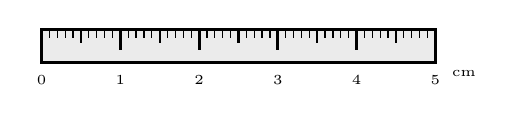
\begin{tikzpicture}[x=1cm, y=1cm, every node/.style={font=\scriptsize, text=black}]
      \draw[black, line width=1.1pt, fill=panelgray] (0,0) rectangle (5.0, 0.42);
      \foreach \m in {0,...,50}{
        \pgfmathsetmacro{\xval}{\m*0.1}
        \draw[black, line width=0.45pt] (\xval, 0.42) -- (\xval, 0.31);
      }
      \foreach \h in {0,0.5,...,5.0}{
        \draw[black, line width=0.8pt] (\h, 0.42) -- (\h, 0.24);
      }
      \foreach \c in {0,1,2,3,4,5}{
        \draw[black, line width=1.1pt] (\c, 0.42) -- (\c, 0.15);
        \node[below=1pt, font=\tiny] at (\c, 0.0) {\en{\c}};
      }
      \node[right=2pt, font=\tiny] at (5.02, -0.14) {\en{cm}};
    \end{tikzpicture}
  \end{tcolorbox}
\end{minipage}

\vspace{3pt}

% --- ផ្នែកទី ១៖ សកម្មភាព 1 — បត់ត្រីកោណសមបាទ ∆ABC (1:1) vs បន្ទះកំពូលខុស ∆PQR (1:1) ---
\textbf{១. សកម្មភាព \en{1} ៖ បត់សមបាទ $\tri{ABC}$ (\en{6.0--5.0--5.0 cm}) \en{vs} កំពូលខុស $\tri{PQR}$ (\en{4.5--4.5--3.0 cm}) (\en{x=1cm, y=1cm})}

\vspace{2pt}
\noindent
\begin{minipage}[c]{7.55cm}
  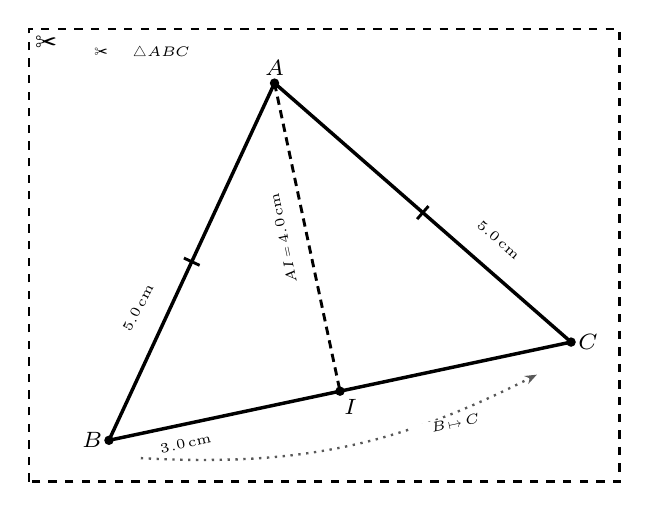
\begin{tikzpicture}[x=1cm, y=1cm, every node/.style={font=\scriptsize, text=black}]
    % Cuttable box: 7.50 cm x 5.75 cm
    \draw[black, dashed, line width=0.95pt] (0, 0) rectangle (7.50, 5.75);
    \node[anchor=north west, inner sep=1pt, font=\footnotesize] at (0.04, 5.71) {\scissors};
    \node[anchor=north west, font=\tiny] at (0.42, 5.65) {\textbf{កាត់ \scissors{} តាម $\tri{ABC}$}};

    % Exact 1:1 tilted 12 deg isosceles ABC: I=(3.95, 1.15), BC=6.0, AI=4.0, AB=AC=5.0
    % u=(0.978148, 0.207912), n=(-0.207912, 0.978148)
    \coordinate (I) at (3.9500, 1.1500);
    \coordinate (B) at (1.0156, 0.5263);
    \coordinate (C) at (6.8844, 1.7737);
    \coordinate (A) at (3.1184, 5.0626);

    % Triangle edges (solid cut line) & crease guide (AI)
    \draw[black, line width=1.25pt] (B) -- (C);
    \draw[black, line width=1.25pt, tk1] (A) -- (B);
    \draw[black, line width=1.25pt, tk1] (A) -- (C);
    \draw[black, densely dashed, line width=1.05pt] (A) -- (I);

    % Fold hint arc B -> C
    \draw[darkline, dotted, line width=0.85pt, -{Stealth[length=1.5mm]}] (1.42, 0.30) to[bend right=15] (6.45, 1.36);
    \node[font=\tiny, fill=white, inner sep=0.6pt, rotate=12] at (5.30, 0.72) {បត់ $B\mapsto C$};

    % Clean labels clear of lines, header, & ticks
    \fill[black] (A) circle (0.06) node[above=2pt, fill=white, inner sep=0.6pt, font=\footnotesize] {$A$};
    \fill[black] (B) circle (0.06) node[left=2pt, fill=white, inner sep=0.6pt, font=\footnotesize] {$B$};
    \fill[black] (C) circle (0.06) node[right=2pt, fill=white, inner sep=0.6pt, font=\footnotesize] {$C$};
    \fill[black] (I) circle (0.06) node[below right=2pt and 1pt, fill=white, inner sep=0.6pt, font=\footnotesize] {$I$};

    \node[font=\tiny, rotate=63, fill=white, inner sep=0.6pt] at ($(A)!0.66!(B)+(-0.34, 0.14)$) {$5.0\unit{cm}$};
    \node[font=\tiny, rotate=-41, fill=white, inner sep=0.6pt] at ($(A)!0.66!(C)+(0.36, 0.18)$) {$5.0\unit{cm}$};
    \node[font=\tiny, rotate=12, fill=white, inner sep=0.6pt] at ($(B)!0.32!(I)+(0.04, -0.24)$) {$3.0\unit{cm}$};
    \node[font=\tiny, rotate=102, fill=white, inner sep=0.6pt] at ($(I)!0.48!(A)+(-0.32, 0.06)$) {$AI=4.0\unit{cm}$};
  \end{tikzpicture}
\end{minipage}%
\hfill
\begin{minipage}[c]{5.50cm}
  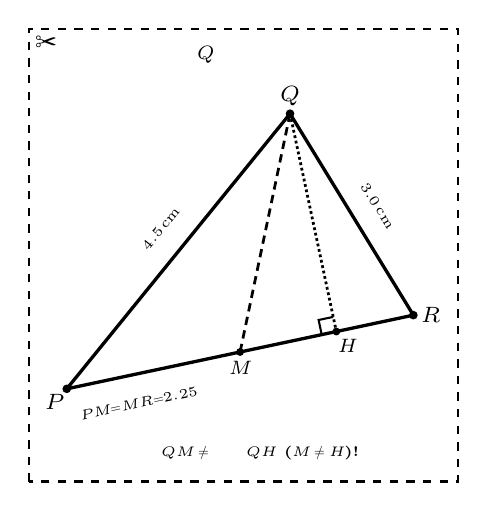
\begin{tikzpicture}[x=1cm, y=1cm, every node/.style={font=\scriptsize, text=black}]
    % Wrong-Apex Control Cutout box: 5.45 cm x 5.75 cm
    \draw[black, dashed, line width=0.95pt] (0, 0) rectangle (5.45, 5.75);
    \node[anchor=north west, inner sep=1pt, font=\footnotesize] at (0.04, 5.71) {\scissors};
    \node[anchor=north west, font=\scriptsize] at (0.42, 5.66) {\textbf{បន្ទះបញ្ឆោត៖ កំពូលខុស $Q$}};

    % Exact 1:1 Isosceles PQR (PQ=PR=4.5 cm, QR=3.0 cm) tested from base vertex Q!
    \coordinate (P) at (0.4800, 1.1800);
    \coordinate (R) at (4.8817, 2.1156);
    \coordinate (M) at (2.6808, 1.6478);
    \coordinate (H) at (3.9035, 1.9077);
    \coordinate (Q) at (3.3154, 4.6743);

    \draw[black, line width=1.2pt] (P) -- (Q) -- (R) -- cycle;
    \draw[black, densely dashed, line width=1.0pt] (Q) -- (M);
    \draw[black, densely dotted, line width=1.0pt] (Q) -- (H);
    \pic[draw=black, line width=0.75pt, angle radius=1.9mm]{right angle=P--H--Q};

    \fill[black] (P) circle (0.055) node[below left=1.5pt, fill=white, inner sep=0.6pt, font=\footnotesize] {$P$};
    \fill[black] (Q) circle (0.055) node[above=2pt, fill=white, inner sep=0.6pt, font=\footnotesize] {$Q$};
    \fill[black] (R) circle (0.055) node[right=2pt, fill=white, inner sep=0.6pt, font=\footnotesize] {$R$};
    \fill[black] (M) circle (0.050) node[below=2.5pt, fill=white, inner sep=0.6pt, font=\scriptsize] {$M$};
    \fill[black] (H) circle (0.050) node[below right=2pt and 0pt, fill=white, inner sep=0.6pt, font=\scriptsize] {$H$};

    \node[font=\tiny, rotate=51, fill=white, inner sep=0.6pt] at ($(P)!0.52!(Q)+(-0.28, 0.22)$) {$4.5\unit{cm}$};
    \node[font=\tiny, rotate=-58, fill=white, inner sep=0.6pt] at ($(Q)!0.52!(R)+(0.30, 0.16)$) {$3.0\unit{cm}$};
    \node[font=\tiny, rotate=12, fill=white, inner sep=0.6pt] at ($(P)!0.38!(M)+(0.08, -0.36)$) {$PM{=}MR{=}2.25$};
    \node[font=\tiny, fill=white, inner sep=0.6pt] at (2.72, 0.36) {\textbf{មេដ្យាន $QM \neq$ កម្ពស់ $QH$ ($M\neq H$)!}};
  \end{tikzpicture}
\end{minipage}%
\hfill
\begin{minipage}[c]{5.65cm}
  \begin{tcolorbox}[
    enhanced, sharp corners, colback=white, colframe=black,
    boxrule=1.0pt, boxsep=1pt, top=3pt, bottom=3pt, left=4.5pt, right=4.5pt,
    title={\textbf{កំណត់ត្រាសកម្មភាព \en{1}}},
    colbacktitle=headgray, coltitle=black, fonttitle=\fontsize{8.0pt}{10.5pt}\selectfont
  ]
    \raggedright\fontsize{7.55pt}{10.5pt}\selectfont
    \textbf{១. បត់ $\tri{ABC}$ ($B\mapsto C$) តាម $(AI)$៖}\\[1.5pt]
    $\bullet$ $IB=\underline{\hspace{0.42cm}}\unit{cm},\; IC=\underline{\hspace{0.42cm}}\unit{cm}$ \chkbox\ $=3.0$\\[1.5pt]
    $\bullet$ $\ang{AIB}=\underline{\hspace{0.40cm}}^\circ$ \chkbox\ $=90^\circ$\\[1.5pt]
    $\bullet$ មុំបាទ $\ang{B}\stackrel{?}{=}\ang{C}$ \chkbox\ ប៉ុនគ្នា\\[1.5pt]
    $\bullet$ ពុះកំពូល $\ang{BAI}\stackrel{?}{=}\ang{CAI}$ \chkbox\ ប៉ុនគ្នា\\[2pt]
    $\Rightarrow (AI)$ ជា\textbf{បន្ទាត់រួម ៤-ក្នុង-១}!\\[3pt]
    \hrule height 0.5pt\vspace{3pt}
    \textbf{២. បន្ទះកំពូលខុស $\tri{PQR}$ (ពី $Q$)៖}\\[1.5pt]
    $QP=4.5\unit{cm} \neq QR=3.0\unit{cm}$; $PM=MR=2.25\unit{cm}$ តែ $PH=3.5\unit{cm}$ ($MH=1.25\unit{cm}$)!\\
    $\Rightarrow$ បត់ $P\mapsto R$ \textbf{មិនត្រួត} — \textbf{៤-ក្នុង-១ កើតតែពីកំពូល $A$!}
  \end{tcolorbox}
\end{minipage}

\vspace{3.5pt}

% --- ផ្នែកទី ២៖ សកម្មភាព 2 (POE) — ប្រសព្វមេដ្យាទ័រ O (មុំស្រួចក្នុង vs មុំទាលក្រៅ, x=1cm, y=1cm) ---
\textbf{២. សកម្មភាព \en{2} (\en{POE}) ៖ ប្រៀបធៀបទីតាំងប្រសព្វមេដ្យាទ័រ មុំស្រួច $\tri{ABC}$ \en{vs} មុំទាល $\tri{DEF}$ ($\ang{E}=115^\circ$) (\en{x=1cm, y=1cm})}

\vspace{2pt}
\noindent
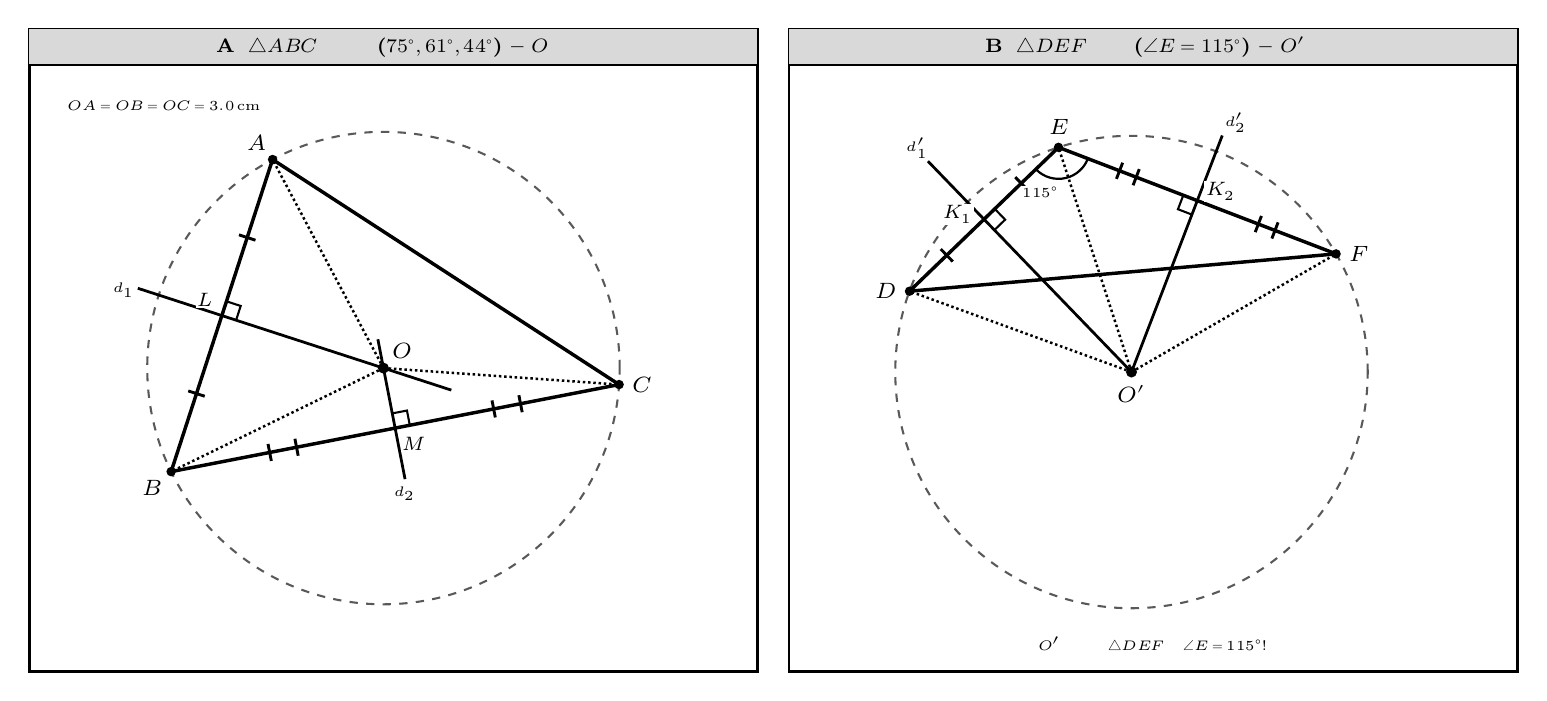
\begin{tikzpicture}[x=1cm, y=1cm, every node/.style={font=\scriptsize, text=black}]
  % === Panel A: Acute Scalene ABC (R=3.00 cm exact, O inside) ===
  \begin{scope}[shift={(0,0)}]
    \draw[black, line width=1.05pt] (0, 0) rectangle (9.25, 8.15);
    \fill[headgray] (0, 7.70) rectangle (9.25, 8.15);
    \draw[black, line width=0.85pt] (0, 7.70) -- (9.25, 7.70);
    \node[font=\scriptsize] at (4.625, 7.925) {\textbf{ផ្ទាំង \en{A}៖ $\tri{ABC}$ មុំស្រួច ($75^\circ, 61^\circ, 44^\circ$) \en{--} $O$ នៅខាងក្នុង}};

    \coordinate (O) at (4.5000, 3.8500);
    \coordinate (A) at (3.0916, 6.4988);
    \coordinate (B) at (1.8036, 2.5349);
    \coordinate (C) at (7.4927, 3.6407);
    \coordinate (L) at ($(A)!0.5!(B)$);
    \coordinate (M) at ($(B)!0.5!(C)$);

    \draw[darkline, dashed, line width=0.75pt] (O) circle (3.00);
    \draw[black, densely dotted, line width=0.9pt] (O) -- (A) (O) -- (B) (O) -- (C);

    \draw[black, line width=1.25pt, tk1] (A) -- (L);
    \draw[black, line width=1.25pt, tk1] (L) -- (B);
    \draw[black, line width=1.25pt, tk2] (B) -- (M);
    \draw[black, line width=1.25pt, tk2] (M) -- (C);
    \draw[black, line width=1.25pt] (A) -- (C);

    \draw[black, line width=1.0pt] ($(O)!-0.42!(L)$) -- ($(O)!1.52!(L)$);
    \draw[black, line width=1.0pt] ($(O)!-0.48!(M)$) -- ($(O)!1.85!(M)$);
    \pic[draw=black, line width=0.75pt, angle radius=1.9mm]{right angle=O--L--A};
    \pic[draw=black, line width=0.75pt, angle radius=1.9mm]{right angle=O--M--C};

    \fill[black] (A) circle (0.06);
    \node[above left=2.5pt and 1.5pt, fill=white, inner sep=0.6pt, font=\footnotesize] at (A) {$A$};
    \fill[black] (B) circle (0.06);
    \node[below left=2.5pt and 2.5pt, fill=white, inner sep=0.6pt, font=\footnotesize] at (B) {$B$};
    \fill[black] (C) circle (0.06);
    \node[right=4pt, fill=white, inner sep=0.6pt, font=\footnotesize] at (C) {$C$};
    \fill[black] (O) circle (0.07);
    \node[above right=2.5pt and 2.5pt, fill=white, inner sep=0.6pt, font=\footnotesize] at (O) {\textbf{$O$}};
    \node[above left=2.5pt and 2.5pt, fill=white, inner sep=0.6pt, font=\scriptsize] at (L) {$L$};
    \node[below right=2.5pt and 2pt, fill=white, inner sep=0.6pt, font=\scriptsize] at (M) {$M$};
    \node[left=3pt, fill=white, inner sep=0.6pt, font=\tiny] at ($(O)!1.48!(L)$) {$d_1$};
    \node[below=3pt, fill=white, inner sep=0.6pt, font=\tiny] at ($(O)!1.80!(M)$) {$d_2$};
    \node[font=\tiny, fill=white, inner sep=0.6pt] at (1.55, 7.18) {វាស់៖ $OA=OB=OC=3.0\unit{cm}$};
  \end{scope}

  % === Panel B: Obtuse DEF (angle E = 115 deg, R=3.00 cm, O' OUTSIDE opposite E) ===
  \begin{scope}[shift={(9.65,0)}]
    \draw[black, line width=1.05pt] (0, 0) rectangle (9.25, 8.15);
    \fill[headgray] (0, 7.70) rectangle (9.25, 8.15);
    \draw[black, line width=0.85pt] (0, 7.70) -- (9.25, 7.70);
    \node[font=\scriptsize] at (4.625, 7.925) {\textbf{ផ្ទាំង \en{B}៖ $\tri{DEF}$ មុំទាល ($\ang{E}=115^\circ$) \en{--} $O'$ នៅខាងក្រៅ}};

    % O'=(4.35, 3.80), R=3.00 -> tD=160, tE=108, tF=30 -> angle E = 115.00 deg exact!
    \coordinate (Op) at (4.3500, 3.8000);
    \coordinate (D) at (1.5309, 4.8261);
    \coordinate (E) at (3.4229, 6.6532);
    \coordinate (F) at (6.9481, 5.3000);
    \coordinate (K1) at ($(D)!0.5!(E)$);
    \coordinate (K2) at ($(E)!0.5!(F)$);

    \draw[darkline, dashed, line width=0.75pt] (Op) circle (3.00);
    \draw[black, densely dotted, line width=0.9pt] (Op) -- (D) (Op) -- (E) (Op) -- (F);

    \draw[black, line width=1.25pt, tk1] (D) -- (K1);
    \draw[black, line width=1.25pt, tk1] (K1) -- (E);
    \draw[black, line width=1.25pt, tk2] (E) -- (K2);
    \draw[black, line width=1.25pt, tk2] (K2) -- (F);
    \draw[black, line width=1.25pt] (D) -- (F);

    % Angle E = 115 deg arc & label cleanly in wide DE--O'E sector (-108 deg)
    \pic[draw=black, line width=0.8pt, angle radius=4.0mm]{angle=D--E--F};
    \node[fill=white, inner sep=0.5pt, font=\tiny] at ($(E)+(-112:0.62)$) {$115^\circ$};

    % Perpendicular bisectors d'_1 & d'_2 meeting cleanly at O' (not extending below O'!)
    \draw[black, line width=1.0pt] (Op) -- ($(Op)!1.38!(K1)$);
    \draw[black, line width=1.0pt] (Op) -- ($(Op)!1.38!(K2)$);
    \pic[draw=black, line width=0.75pt, angle radius=1.9mm]{right angle=Op--K1--E};
    \pic[draw=black, line width=0.75pt, angle radius=1.9mm]{right angle=Op--K2--E};

    \fill[black] (D) circle (0.06);
    \node[left=4pt, fill=white, inner sep=0.6pt, font=\footnotesize] at (D) {$D$};
    \fill[black] (E) circle (0.06);
    \node[above=4pt, fill=white, inner sep=0.6pt, font=\footnotesize] at (E) {$E$};
    \fill[black] (F) circle (0.06);
    \node[right=4pt, fill=white, inner sep=0.6pt, font=\footnotesize] at (F) {$F$};
    \fill[black] (Op) circle (0.07);
    \node[below=4pt, fill=white, inner sep=0.6pt, font=\footnotesize] at (Op) {\textbf{$O'$}};
    \node[fill=white, inner sep=0.6pt, font=\scriptsize] at ($(K1)+(170:0.34)$) {$K_1$};
    \node[fill=white, inner sep=0.6pt, font=\scriptsize] at ($(K2)+(22:0.32)$) {$K_2$};
    \node[above left=2pt and 1pt, fill=white, inner sep=0.6pt, font=\tiny] at ($(Op)!1.35!(K1)$) {$d'_1$};
    \node[above right=2pt and 1pt, fill=white, inner sep=0.6pt, font=\tiny] at ($(Op)!1.35!(K2)$) {$d'_2$};
    \node[font=\tiny, fill=white, inner sep=0.6pt] at (4.62, 0.35) {$O'$ នៅ\textbf{ខាងក្រៅ} $\tri{DEF}$ ឈម $\ang{E}=115^\circ$!};
  \end{scope}
\end{tikzpicture}

\vspace{3pt}
\begin{tcolorbox}[
  enhanced, sharp corners, colback=white, colframe=black,
  boxrule=0.95pt, boxsep=1pt, top=3pt, bottom=3pt, left=5pt, right=5pt
]
  \raggedright\fontsize{7.7pt}{10.8pt}\selectfont
  \textbf{\en{P} -- ទស្សន៍ទាយមុនវាស់៖} បើ $\tri{DEF}$ មានមុំទាល $115^\circ$ តើប្រសព្វមេដ្យាទ័រ $O'$ ស្ថិតនៅឯណា? \chkbox\ ក្នុង \chkbox\ លើជ្រុង \chkbox\ ខាងក្រៅ (ឈម $115^\circ$)\\[2.5pt]
  \textbf{\en{O} -- តារាងផ្ទៀងវាស់ខ្នាត \en{1:1} ជាមួយបន្ទាត់ \en{cm}៖}\\[1.5pt]
  \renewcommand{\arraystretch}{1.12}
  \begin{tabular}{|L{4.80cm}|L{8.45cm}|L{4.15cm}|}
    \hline
    \cellcolor{headgray}\textbf{រូបគំរូ \en{POE}} & \cellcolor{headgray}\textbf{រង្វាស់ចម្ងាយពីប្រសព្វទៅកំពូលទាំង ៣ (\en{cm})} & \cellcolor{headgray}\textbf{ទីតាំងប្រសព្វ} \\ \hline
    ផ្ទាំង \en{A}៖ $\tri{ABC}$ មុំស្រួច & $OA=\underline{\hspace{0.55cm}}\unit{cm},\quad OB=\underline{\hspace{0.55cm}}\unit{cm},\quad OC=\underline{\hspace{0.55cm}}\unit{cm}$ & \chkbox\ ក្នុង $\tri{ABC}$ \quad \chkbox\ ក្រៅ \\ \hline
    ផ្ទាំង \en{B}៖ $\tri{DEF}$ ($\ang{E}=115^\circ$) & $O'D=\underline{\hspace{0.55cm}}\unit{cm},\quad O'E=\underline{\hspace{0.55cm}}\unit{cm},\quad O'F=\underline{\hspace{0.55cm}}\unit{cm}$ & \chkbox\ ក្នុង \quad \chkbox\ ក្រៅ $\tri{DEF}$ \\ \hline
  \end{tabular}\\[3pt]
  \textbf{\en{E} -- ពន្យល់៖} ហេតុអ្វីទោះ $O'$ ស្ថិតនៅខាងក្រៅ $\tri{DEF}$ ក៏ $O'D=O'E=O'F$ ($=3.0\unit{cm}$) នៅតែស្មើគ្នា (តាមទ្រឹស្ដីបទមេដ្យាទ័រ)? $\underline{\hspace{3.6cm}}$
\end{tcolorbox}

\clearpage

% ============================================================================
% ទំព័រទី ២៖ E4 Elaborate — ២ ប័ណ្ណ "ផែនទីច្រវាក់ប្រសព្វមេដ្យាទ័រ និងបន្ទាត់ ៤-ក្នុង-១"
% ============================================================================
\pagebanner{សម្ភារៈទី ២៖ កាត \enbf{E4} «ផែនទីច្រវាក់ប្រសព្វមេដ្យាទ័រ និងបន្ទាត់ ៤\enbf{-}ក្នុង\enbf{-}១»}{ទំព័រ ២/៦ \en{-- E4 Elaborate} (កាត់ ២ ប័ណ្ណ \scissors)}

\newcommand{\eFourCardISO}[1]{%
\begin{tcolorbox}[
  enhanced, sharp corners, colback=white, colframe=white,
  borderline={1.0pt}{0pt}{black, dashed},
  boxsep=1pt, top=3.5pt, bottom=3.5pt, left=5pt, right=5pt
]
  \begin{tcolorbox}[
    enhanced, sharp corners, colback=headgray, colframe=black,
    boxrule=0.8pt, boxsep=1pt, top=2.5pt, bottom=2.5pt, left=5pt, right=5pt, after skip=4pt
  ]
    \fontsize{8.2pt}{11.0pt}\selectfont
    \textbf{\scissors\ កាត \en{E4} (#1) \en{--} ផែនទីច្រវាក់ប្រសព្វមេដ្យាទ័រ និងបន្ទាត់ ៤-ក្នុង-១} \hfill ក្រុម៖ $\underline{\hspace{2.6cm}}$
  \end{tcolorbox}

  \noindent
  \begin{minipage}[t]{7.55cm}
    \vspace{0pt}
    \fontsize{7.7pt}{10.8pt}\selectfont
    \textbf{លំហាត់គំរូ \en{E4} (សៀវភៅទំ.១៥៧ -- រូបកែតម្រូវ)៖} មេដ្យាទ័រនៃជ្រុង $AB$ និង $BC$ នៃ $\tri{ABC}$ ប្រសព្វគ្នាត្រង់ $O$។ \textbf{(ក)} បង្ហាញថា $OA=OB=OC$។ \textbf{(ខ)} បើ $N$ ជាចំណុចកណ្ដាលនៃ $AC$ បង្ហាញថា $ON\perp AC$។
    \begin{center}
    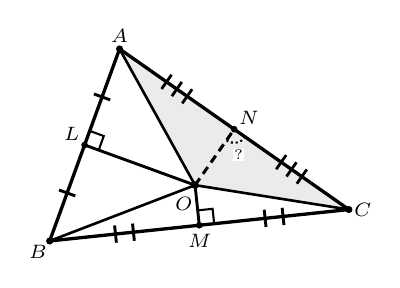
\begin{tikzpicture}[scale=0.86, every node/.style={font=\scriptsize, text=black}]
      % Scalene acute ABC (angles ~75, 64, 41): A-O-M & B-O-N visibly NON-collinear!
      % NO 90 deg square at N! Dashed ON with '?' at N!
      \coordinate (O) at (2.2500, 1.3500);
      \coordinate (A) at (1.1349, 3.3616);
      \coordinate (B) at (0.1028, 0.5258);
      \coordinate (C) at (4.5217, 0.9902);
      \coordinate (L) at ($(A)!0.5!(B)$);
      \coordinate (M) at ($(B)!0.5!(C)$);
      \coordinate (N) at ($(A)!0.5!(C)$);

      \fill[panelgray] (O) -- (A) -- (C) -- cycle;

      \draw[black, line width=1.2pt, tk1] (A) -- (L);
      \draw[black, line width=1.2pt, tk1] (L) -- (B);
      \draw[black, line width=1.2pt, tk2] (B) -- (M);
      \draw[black, line width=1.2pt, tk2] (M) -- (C);
      \draw[black, line width=1.2pt, tk3] (A) -- (N);
      \draw[black, line width=1.2pt, tk3] (N) -- (C);

      \draw[black, line width=0.95pt] (O) -- (A) (O) -- (B) (O) -- (C);
      \draw[black, line width=1.05pt] (O) -- (L) (O) -- (M);
      \pic[draw=black, line width=0.75pt, angle radius=1.9mm]{right angle=O--L--A};
      \pic[draw=black, line width=0.75pt, angle radius=1.9mm]{right angle=O--M--C};

      % Dashed ON with exact dotted angle arc between NO (-125 deg) and NC (-35 deg)
      \draw[black, densely dashed, line width=1.1pt] (O) -- (N);
      \draw[black, densely dotted, line width=0.75pt] ($(N)+(-125:0.20)$) arc (-125:-35:0.20);
      \node[font=\tiny, fill=white, inner sep=0.4pt] at ($(N)+(-80:0.38)$) {$?$};

      \fill[black] (A) circle (1.5pt) node[above=1.5pt, fill=white, inner sep=0.5pt] {$A$};
      \fill[black] (B) circle (1.5pt) node[below left=1pt, fill=white, inner sep=0.5pt] {$B$};
      \fill[black] (C) circle (1.5pt) node[right=1.5pt, fill=white, inner sep=0.5pt] {$C$};
      \fill[black] (L) circle (1.4pt) node[above left=1.5pt, fill=white, inner sep=0.5pt] {$L$};
      \fill[black] (M) circle (1.4pt) node[below=2.5pt, fill=white, inner sep=0.5pt] {$M$};
      \fill[black] (N) circle (1.4pt) node[above right=1.5pt, fill=white, inner sep=0.5pt] {$N$};
      % Place O cleanly inside the 75 deg open sector between OB (201) and OM (276)
      \fill[black] (O) circle (1.6pt);
      \node[fill=white, inner sep=0.5pt] at ($(O)+(238:0.32)$) {$O$};
    \end{tikzpicture}
    \end{center}
    \begin{tcolorbox}[enhanced, sharp corners, colback=panelgray, colframe=black, boxrule=0.7pt, boxsep=1pt, top=2.5pt, bottom=2.5pt, left=4pt, right=4pt]
      \raggedright\fontsize{7.2pt}{10.0pt}\selectfont
      \textbf{ពិនិត្យក្រោយ (\en{EIA} ៣០ វិនាទី)៖ ហេតុអ្វី $ON$ មិនកាត់កំពូល $B$?}\\
      ព្រោះ $\tri{ABC}$ ជាត្រីកោណ\textbf{សាមញ្ញ} ($BA\neq BC$)៖ $ON$ ជាមេដ្យាទ័រ $AC$ ក្នុង $\tri{OAC}$ ($OA=OC$) ប៉ុន្តែ $B$ មិនស្មើចម្ងាយពី $A, C$ ទេ!
    \end{tcolorbox}
  \end{minipage}\hfill
  \begin{minipage}[t]{10.25cm}
    \vspace{0pt}
    \begin{tcolorbox}[enhanced, sharp corners, colback=white, colframe=black, boxrule=0.85pt, boxsep=1pt, top=3pt, bottom=3pt, left=5pt, right=5pt]
      \raggedright\fontsize{7.65pt}{10.8pt}\selectfont
      \textbf{(ក) បង្ហាញថា $OA=OB=OC$ [\en{[tracing]} តាម $OA, OB, OC$]៖}\\
      \chkbox\ អូសម្រាមដៃ \en{[tracing]} តាមអង្កត់ $OA, OB, OC$ លើរូប៖\\
      $\bullet$ មេដ្យាទ័រ $AB$ កាត់ $AB$ ត្រង់ $L$ ($AL=LB$ \tickone, $90^\circ$) និង $O$ ស្ថិតនៅលើ $(OL)$ $\Rightarrow OA = \underline{\hspace{0.55cm}}$ (\cnum{4})\\
      $\bullet$ មេដ្យាទ័រ $BC$ កាត់ $BC$ ត្រង់ $M$ ($BM=MC$ \ticktwo, $90^\circ$) និង $O$ ស្ថិតនៅលើ $(OM)$ $\Rightarrow OB = \underline{\hspace{0.55cm}}$ (\cnum{4})\\
      ដូចនេះ $OA = OB = \underline{\hspace{0.55cm}}$~។
    \end{tcolorbox}
    \vspace{2.5pt}
    \begin{tcolorbox}[enhanced, sharp corners, colback=panelgray, colframe=black, boxrule=0.85pt, boxsep=1pt, top=3pt, bottom=3pt, left=5pt, right=5pt]
      \raggedright\fontsize{7.65pt}{10.8pt}\selectfont
      \textbf{(ខ) បង្ហាញថា $ON\perp AC$ [\en{[tracing]} $\tri{OAC}$ \en{+} ៤-ក្នុង-១]៖}\\
      \chkbox\ អូសម្រាមដៃជុំវិញ $\tri{OAC}$ (ផ្ទៃប្រផេះ)៖\\
      $\bullet$ តាម \textbf{(ក)}៖ $OA = OC \Rightarrow \tri{OAC}$ ជាត្រីកោណ\textbf{សមបាទកំពូល $\underline{\hspace{0.45cm}}$} (\cnum{1})\\
      $\bullet$ $N$ ជាចំណុចកណ្ដាល $AC$ ($AN=NC$ \tickthree) $\Rightarrow ON$ ជា\textbf{មេដ្យាន}ចេញពីកំពូល $O$ នៃ $\tri{OAC}$\\
      $\bullet$ តាមបន្ទាត់ ៤-ក្នុង-១ ពីកំពូល $O$ (\cnum{3}) $\Rightarrow ON$ ជាមេដ្យាទ័រ/កម្ពស់ $\Rightarrow ON \underline{\hspace{0.48cm}} AC$ ($90^\circ$)!
    \end{tcolorbox}
    \vspace{2.5pt}
    \raggedright{\fontsize{6.8pt}{9.4pt}\selectfont
    \textbf{ធនាគារ \cnum{1}--\cnum{5}៖} \cnum{1} ផ្ទាល់សមបាទ \en{|} \cnum{2} ច្រាស \en{|} \cnum{3} ៤-ក្នុង-១ កំពូល \en{|} \cnum{4} មេដ្យាទ័រ/ប្រសព្វ $O$ \en{|} \cnum{5} ប៉ុនគ្នា/$180^\circ$\par}
  \end{minipage}
\end{tcolorbox}%
}

\eFourCardISO{ប័ណ្ណទី ១}

\vspace{5.5pt}
\noindent\scissors\ \dotfill\ \textbf{កាត់តាមស្នាមចុចចែកជា ២ ប័ណ្ណ (\en{Cut Along Dashed Line})} \dotfill\ \scissors
\vspace{5.5pt}

\eFourCardISO{ប័ណ្ណទី ២}

\clearpage

% ============================================================================
% ទំព័រទី ៣៖ E5 Evaluate — "តុផ្ទៀងផ្ទាត់មុំបាទ និងប៉មទឹកសហគមន៍ ៣ តួនាទី" ប្រតិបត្តិ (២ សន្លឹក)
% ============================================================================
\pagebanner{សម្ភារៈទី ៣៖ «តុផ្ទៀងផ្ទាត់មុំបាទ និងប៉មទឹកសហគមន៍ ៣ តួនាទី» \enbf{--} ប្រតិបត្តិ \enbf{(E5 \& E1)}}{ទំព័រ ៣/៦ \en{-- E5 Evaluate} (កាត់ ២ សន្លឹក \scissors)}

\newcommand{\eFiveSheetISO}[1]{%
\begin{tcolorbox}[
  enhanced, sharp corners, colback=white, colframe=white,
  borderline={1.0pt}{0pt}{black, dashed},
  boxsep=1pt, top=2pt, bottom=2pt, left=4.5pt, right=4.5pt
]
  \begin{tcolorbox}[
    enhanced, sharp corners, colback=headgray, colframe=black,
    boxrule=0.8pt, boxsep=1pt, top=1.5pt, bottom=1.5pt, left=4pt, right=4pt, after skip=2pt
  ]
    \fontsize{6.85pt}{9.2pt}\selectfont
    \textbf{\scissors\ តុផ្ទៀង ៣ តួនាទី (#1)} \en{|} ក្រុម៖ $\underline{\hspace{0.85cm}}$ \hfill \textbf{(ក)} ហោជាង $AB{=}AC, \ang{A}{=}50^\circ, AI\perp BC, BC{=}10\unit{m}$ \en{|} \textbf{(ខ)} ផ្លូវកោង $\ang{B}{=}110^\circ$, ប៉ម $O$: $OA{=}2x{+}3,\; OC{=}5x{-}12$
  \end{tcolorbox}

  \renewcommand{\arraystretch}{1.01}
  {\centering\setlength{\tabcolsep}{3.5pt}%
  \begin{tabular}{|L{6.55cm}|L{5.85cm}|L{5.20cm}|}
    \hline
    \cellcolor{panelgray}\centering\arraybackslash\fontsize{7.2pt}{9.4pt}\selectfont\textbf{តួនាទី ១៖ គូសសញ្ញា \en{\&} \en{Pause-Ask!}}\newline {\fontsize{6.5pt}{8.5pt}\selectfont សម្គាល់ \tickone\ លើ $AB{=}AC$, $90^\circ$ ត្រង់ $I$, និង $O$ ខាងក្រៅ} &
    \cellcolor{panelgray}\centering\arraybackslash\fontsize{7.2pt}{9.4pt}\selectfont\textbf{តួនាទី ២៖ សម្រាយ \cnum{1}--\cnum{4} \en{\&} ពិជគណិត}\newline {\fontsize{6.5pt}{8.5pt}\selectfont រក $\ang{B}, \ang{BAI}, BI$ (ក) និង $x, OA{=}OB{=}OC$ (ខ)} &
    \cellcolor{panelgray}\centering\arraybackslash\fontsize{7.2pt}{9.4pt}\selectfont\textbf{តួនាទី ៣៖ \en{Pause-Review!} \en{\&} បិទ \en{E1}}\newline {\fontsize{6.5pt}{8.5pt}\selectfont ផ្ទៀង $x=5$ \en{\&} ទីតាំងប៉ម $O$ ក្រៅ $\tri{ABC}$} \\ \hline

    % --- Column 1: Dual Diagram (a) Roof Gable & (b) Obtuse 110 deg 3-House Water Tower ---
    {\centering
    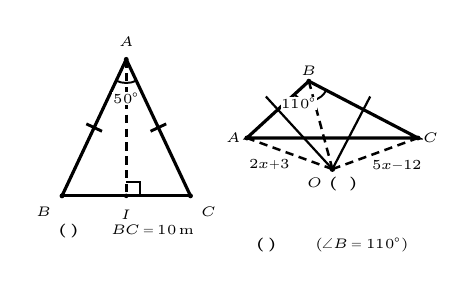
\begin{tikzpicture}[baseline={([yshift=-1ex]current bounding box.north)}, scale=0.68, every node/.style={font=\tiny, text=black}]
      % Left sub-figure (a): Gable ABC (AB=AC, A=50 deg, BC=10 m, AI perp BC)
      \begin{scope}[shift={(0, 0.25)}]
        \coordinate (B1) at (0.0, 0.0);
        \coordinate (C1) at (2.4, 0.0);
        \coordinate (I1) at (1.2, 0.0);
        \coordinate (A1) at (1.2, 2.55);
        \draw[black, line width=1.15pt] (B1) -- (C1);
        \draw[black, line width=1.15pt, tk1] (A1) -- (B1);
        \draw[black, line width=1.15pt, tk1] (A1) -- (C1);
        \draw[black, densely dashed, line width=0.95pt] (A1) -- (I1);
        \pic[draw=black, line width=0.7pt, angle radius=1.8mm]{right angle=C1--I1--A1};
        \pic[draw=black, line width=0.7pt, angle radius=3.0mm]{angle=B1--A1--C1};
        \node[fill=white, inner sep=0.4pt] at (1.2, 1.82) {$50^\circ$};
        \fill[black] (A1) circle (1.3pt) node[above=1pt] {$A$};
        \fill[black] (B1) circle (1.3pt) node[below left=0.5pt] {$B$};
        \fill[black] (C1) circle (1.3pt) node[below right=0.5pt] {$C$};
        \fill[black] (I1) circle (1.2pt) node[below=1.5pt] {$I$};
        \node[below=5pt] at (1.2, -0.08) {\textbf{(ក)} ហោជាង $BC=10\unit{m}$};
      \end{scope}

      % Right sub-figure (b): Obtuse 110 deg Water Tower O outside
      \begin{scope}[shift={(3.25, 0.25)}]
        \coordinate (O2) at (1.8000, 0.5000);
        \coordinate (A2) at (0.2025, 1.0814);
        \coordinate (B2) at (1.3600, 2.1422);
        \coordinate (C2) at (3.3975, 1.0814);
        \coordinate (L2) at ($(A2)!0.5!(B2)$);
        \coordinate (M2) at ($(B2)!0.5!(C2)$);
        \draw[black, line width=1.15pt] (A2) -- (B2) -- (C2) -- cycle;
        \draw[black, line width=0.8pt] (O2) -- ($(O2)!1.22!(L2)$);
        \draw[black, line width=0.8pt] (O2) -- ($(O2)!1.22!(M2)$);
        \draw[black, densely dashed, line width=0.9pt] (O2) -- (A2) (O2) -- (B2) (O2) -- (C2);
        \pic[draw=black, line width=0.7pt, angle radius=2.5mm]{angle=A2--B2--C2};
        % Place 110 deg cleanly in BA--BO open sector (-114 deg)
        \node[fill=white, inner sep=0.3pt] at ($(B2)+(-114:0.46)$) {$110^\circ$};
        \fill[black] (A2) circle (1.3pt) node[left=1.5pt, fill=white, inner sep=0.3pt] {$A$};
        \fill[black] (B2) circle (1.3pt) node[above=1.5pt, fill=white, inner sep=0.3pt] {$B$};
        \fill[black] (C2) circle (1.3pt) node[right=1.5pt, fill=white, inner sep=0.3pt] {$C$};
        \fill[black] (O2) circle (1.5pt) node[below=2.5pt, fill=white, inner sep=0.3pt] {\textbf{$O$ (ប៉ម)}};
        \node[fill=white, inner sep=0.3pt] at ($(O2)!0.52!(A2)+(-0.34,-0.22)$) {$2x{+}3$};
        \node[fill=white, inner sep=0.3pt] at ($(O2)!0.52!(C2)+(0.38,-0.22)$) {$5x{-}12$};
        \node[below=5pt] at (1.80, -0.35) {\textbf{(ខ)} ផ្ទះ ៣ ($\ang{B}=110^\circ$)};
      \end{scope}
    \end{tikzpicture}\par\vspace{1pt}}
    \fontsize{7.0pt}{9.6pt}\selectfont
    \chkbox\ \textbf{\en{Pause-Ask!}} ១) ហេតុអ្វី $AI\perp BC$ ចេញពី $A$ ពុះ $BC$ និង $\ang{A}$? ២) ហេតុអ្វី $O$ ចេញក្រៅ $\tri{ABC}$ ពេល $\ang{B}=110^\circ$?
    &
    % --- Column 2: Solutions (a) and (b) ---
    \fontsize{7.15pt}{10.1pt}\selectfont
    \textbf{(ក) ហោជាងសាលាឆទាន ($\tri{ABC}$ សមបាទ)៖}\par\vspace{1.5pt}
    $\bullet$ $AB=AC \Rightarrow \ang{B}=\ang{C}=\dfrac{180^\circ-50^\circ}{2}=\underline{\hspace{0.48cm}}^\circ$ (\cnum{1}, \cnum{5})\par\vspace{1.5pt}
    $\bullet$ $AI\perp BC$ ពីកំពូល $A \Rightarrow AI$ ជា ៤-ក្នុង-១ (\cnum{3})៖\newline
    $\ang{BAI}=\dfrac{50^\circ}{2}=\underline{\hspace{0.40cm}}^\circ,\; BI=IC=\underline{\hspace{0.40cm}}\unit{m}$\par\vspace{2.5pt}
    \textbf{(ខ) ប៉មទឹកសហគមន៍ ($O$ ប្រសព្វមេដ្យាទ័រ)៖}\par\vspace{1.5pt}
    $\bullet$ $OA=OB=OC$ (\cnum{4}) $\Rightarrow 2x+3=5x-12$\newline
    $\Rightarrow 3x=\underline{\hspace{0.45cm}} \Rightarrow x=\underline{\hspace{0.40cm}} \Rightarrow OA=OB=OC=\underline{\hspace{0.48cm}}\unit{m}$\par\vspace{2.5pt}
    \begin{tcolorbox}[enhanced, sharp corners, colback=panelgray, colframe=black, boxrule=0.65pt, boxsep=1pt, top=2pt, bottom=2pt, left=4pt, right=4pt]
      \raggedright\fontsize{6.75pt}{9.2pt}\selectfont
      \textbf{ធនាគារ៖} \cnum{1} ផ្ទាល់ \en{|} \cnum{3} ៤-ក្នុង-១ \en{|} \cnum{4} ប្រសព្វ $O$ \en{|} \cnum{5} $180^\circ$
    \end{tcolorbox}
    &
    % --- Column 3: Pause-Review & E1 Closure ---
    \fontsize{7.1pt}{10.0pt}\selectfont
    \chkbox\ \textbf{\en{Pause-Review!}} ផ្ទៀង $x=5$៖\newline
    $OA=2(5)+3=\underline{\hspace{0.42cm}}\unit{m}$;\quad $OC=5(5)-12=\underline{\hspace{0.42cm}}\unit{m}$!\par\vspace{2.5pt}
    \chkbox\ ផ្ទៀងទីតាំង៖ ព្រោះ $\ang{B}=110^\circ > 90^\circ$ $\Rightarrow$ ប៉ម $O$ ស្ថិតនៅ\textbf{ខាងក្រៅ} $\tri{ABC}$ ឈមមុំ $B$ តែស្មើចម្ងាយ $13\unit{m}$ ពីផ្ទះ $A, B, C$!\par\vspace{3pt}
    \begin{tcolorbox}[enhanced, sharp corners, colback=panelgray, colframe=black, boxrule=0.7pt, boxsep=1pt, top=2.5pt, bottom=2.5pt, left=4pt, right=4pt]
      \raggedright\fontsize{6.75pt}{9.2pt}\selectfont
      \textbf{បិទបេសកកម្ម \en{E1} (ហោជាង \en{\&} ប៉មទឹក)៖}\\
      ខ្សែប្រយោលកែង $AI$ ពីកំពូល $A$ ពុះហោជាង $\ang{A}=50^\circ$ និង $BC=10\unit{m}$ ស្មើគ្នា ($25^\circ, 5\unit{m}$); ឯប្រសព្វមេដ្យាទ័រ $O$ កំណត់ទីតាំងប៉មទឹកនៅខាងក្រៅផ្លូវកោង $110^\circ$ ចម្ងាយ $13\unit{m}$ ស្មើពីផ្ទះទាំង ៣!
    \end{tcolorbox}
    \\ \hline
  \end{tabular}\par}
\end{tcolorbox}%
}

\eFiveSheetISO{សន្លឹកទី ១}

\vspace{3pt}
\noindent\scissors\ \dotfill\ \textbf{កាត់តាមស្នាមចុចចែកជា ២ សន្លឹក (\en{Cut Along Dashed Line})} \dotfill\ \scissors
\vspace{3pt}

\eFiveSheetISO{សន្លឹកទី ២}

\clearpage

% ============================================================================
% ទំព័រទី ៤៖ ផ្ទាំងយោងប្រចាំថ្នាក់រៀន — ត្រីកោណសមបាទ, ប្រសព្វមេដ្យាទ័រ & ធនាគារ ①–⑤
% ============================================================================
\begin{tcolorbox}[
  enhanced, sharp corners, colback=white, colframe=black,
  boxrule=1.5pt, borderline={0.6pt}{2.2pt}{black},
  boxsep=1pt, top=7pt, bottom=7pt, left=6pt, right=6pt
]
  \begin{center}
    {\muol\fontsize{11.4pt}{16.5pt}\selectfont ទ្រឹស្ដីបទត្រីកោណសមបាទ \enbf{(}ផ្ទាល់\enbf{,} ច្រាស\enbf{,} ៤\enbf{-}ក្នុង\enbf{-}១\enbf{)} និងប្រសព្វមេដ្យាទ័រ \cnum{1}\enbf{--}\cnum{5}}\\[2pt]
    {\fontsize{8.8pt}{12.0pt}\selectfont ផ្ទាំងយោងប្រចាំថ្នាក់រៀន (ស-ខ្មៅ) \en{--} មេរៀនទី១២ (២.២) លក្ខណៈត្រីកោណសមបាទ និងប្រសព្វមេដ្យាទ័រ (ទំ.១៥៧--១៥៨)}\\[3pt]
    \khmflourish
  \end{center}
  \vspace{4pt}

  % --- ផ្នែកទី ១៖ ប្រអប់ផ្ទាល់ + ៤-ក្នុង-១ (ឆ្វេង) & ប្រអប់ច្រាស ម.ជ.ម + ប្រសព្វមេដ្យាទ័រ (ស្ដាំ) ---
  \noindent
  \begin{minipage}[t]{8.95cm}
    \begin{tcolorbox}[enhanced, sharp corners, colback=white, colframe=black, boxrule=0.95pt, boxsep=1pt, equal height group=posterTopISO, top=5pt, bottom=5pt, left=5pt, right=5pt]
      \textbf{\fontsize{8.2pt}{11.2pt}\selectfont លក្ខណៈផ្ទាល់ និងបន្ទាត់រួម ៤-ក្នុង-១ (ចេញពីកំពូល $A$ ប៉ុណ្ណោះ)៖}\\[4pt]
      \begin{minipage}[c]{3.15cm}
        \centering
        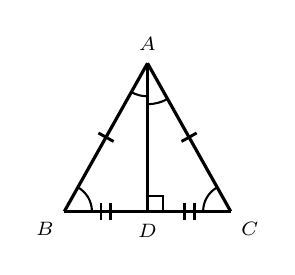
\begin{tikzpicture}[scale=0.66, every node/.style={font=\scriptsize, text=black}]
          \coordinate (B) at (0,0); \coordinate (C) at (3.2,0); \coordinate (D) at (1.6,0); \coordinate (A) at (1.6,2.85);
          \draw[black, line width=1.15pt, tk1] (A)--(B);
          \draw[black, line width=1.15pt, tk1] (A)--(C);
          \draw[black, line width=1.15pt, tk2] (B)--(D);
          \draw[black, line width=1.15pt, tk2] (D)--(C);
          \draw[black, line width=1.05pt] (A)--(D);
          \pic[draw=black, line width=0.75pt, angle radius=2.0mm]{right angle=C--D--A};
          \pic[draw=black, line width=0.75pt, angle radius=3.5mm]{angle=C--B--A};
          \pic[draw=black, line width=0.75pt, angle radius=3.5mm]{angle=A--C--B};
          \pic[draw=black, line width=0.75pt, angle radius=4.2mm]{angle=B--A--D};
          \pic[draw=black, line width=0.75pt, angle radius=5.2mm]{angle=D--A--C};
          \node[above=1pt] at (A) {$A$};
          \node[below left=0.5pt] at (B) {$B$};
          \node[below right=0.5pt] at (C) {$C$};
          \node[below=1pt] at (D) {$D$};
        \end{tikzpicture}
      \end{minipage}\hfill
      \begin{minipage}[c]{5.15cm}
        \raggedright\fontsize{7.7pt}{11.0pt}\selectfont
        $\bullet$ \textbf{ផ្ទាល់ ($AB=AC$)} $\Rightarrow$ មុំបាទ $\ang{B}=\ang{C}$ (តាម $\tri{ABD}\cg\tri{ACD}$, ជ.ម.ជ)~។\\[3pt]
        $\bullet$ \textbf{៤-ក្នុង-១ (ពីកំពូល $A$)៖} មេដ្យាទ័រ, មេដ្យាន, កម្ពស់ និងពុះមុំកំពូល $A$ \textbf{ស្ថិតនៅលើបន្ទាត់ $AD$ តែមួយ}~។\\[3pt]
        $\bullet$ \textbf{ប្រយ័ត្ន៖} មិនកើតពីកំពូលបាត $B, C$ ឬត្រីកោណសាមញ្ញទេ!
      \end{minipage}
    \end{tcolorbox}
  \end{minipage}\hfill
  \begin{minipage}[t]{8.85cm}
    \begin{tcolorbox}[enhanced, sharp corners, colback=panelgray, colframe=black, boxrule=0.95pt, boxsep=1pt, equal height group=posterTopISO, top=5pt, bottom=5pt, left=5pt, right=5pt]
      \raggedright\fontsize{7.7pt}{11.0pt}\selectfont
      \textbf{ទ្រឹស្ដីបទច្រាស (បំពេញទំ.១៥៧) \& ប្រសព្វមេដ្យាទ័រ (ទំ.១៥៨)៖}\\
      $\bullet$ \textbf{ច្រាស ($\ang{B}=\ang{C}\Rightarrow AB=AC$)៖} គូស $AD$ ពុះ $\ang{A}$ ($D\in BC$) $\Rightarrow$ $\ang{BAD}=\ang{CAD}$, $\ang{B}=\ang{C}$, និង $\ang{ADB}=\ang{ADC}$ (ផលបូក $180^\circ$); ជ្រុងរួម $AD \Rightarrow \tri{ABD}\cg\tri{ACD}$ (\textbf{ម.ជ.ម}) $\Rightarrow AB=AC$~។\\[3pt]
      $\bullet$ \textbf{ប្រសព្វមេដ្យាទ័រ (ទំ.១៥៨ កែតម្រូវ)៖} «មេដ្យាទ័រជ្រុងទាំងបីនៃត្រីកោណមួយប្រសព្វគ្នាត្រង់ចំណុចតែមួយ ($O$) ដែល\textbf{ស្ថិតនៅ}ស្មើចម្ងាយពីកំពូលទាំងបីនៃត្រីកោណនោះ ($OA=OB=OC$)\textbf{។}» \textit{(កែពាក្យទំ.១៥៧ «មេដ្យានទ័រ» $\to$ «\textbf{មេដ្យាទ័រ}» និងបន្ថែម «។»!)}
    \end{tcolorbox}
  \end{minipage}

  \vspace{6pt}

  % --- ផ្នែកទី ២៖ តារាងធនាគារអំណះអំណាង ①–⑤ (ស៊ីគ្នា ១០០% នឹង LS_Plan_ISO) ---
  \fontsize{7.9pt}{11.2pt}\selectfont
  \renewcommand{\arraystretch}{1.18}
  \begin{tabular}{|C{0.68cm}|L{4.55cm}|L{6.55cm}|C{4.40cm}|}
    \hline
    \cellcolor{headgray}\textbf{លេខ} &
    \cellcolor{headgray}\centering\arraybackslash\textbf{ឈ្មោះអំណះអំណាង} &
    \cellcolor{headgray}\centering\arraybackslash\textbf{និមិត្តសញ្ញា និងរបៀបប្រើ} &
    \cellcolor{headgray}\centering\arraybackslash\textbf{រូបសម្គាល់ ស-ខ្មៅ} \\ \hline

    \cnum{1} &
    \textbf{លក្ខណៈផ្ទាល់ត្រីកោណសមបាទ} &
    $AB=AC \Rightarrow \ang{B}=\ang{C}$ (មុំបាទទាំងពីរជាមុំប៉ុនគ្នា)~។ &
    \raisebox{-0.35\height}{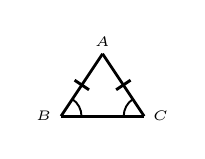
\begin{tikzpicture}[scale=0.48, every node/.style={font=\tiny, text=black}]
      \coordinate (b) at (0,0); \coordinate (c) at (2.2,0); \coordinate (a) at (1.1,1.65);
      \draw[black, line width=1.0pt, tk1] (a)--(b); \draw[black, line width=1.0pt, tk1] (a)--(c); \draw[black, line width=1.0pt] (b)--(c);
      \pic[draw=black, line width=0.7pt, angle radius=2.6mm]{angle=c--b--a};
      \pic[draw=black, line width=0.7pt, angle radius=2.6mm]{angle=a--c--b};
      \node[above=-1pt] at (a) {$A$}; \node[left=0pt] at (b) {$B$}; \node[right=0pt] at (c) {$C$};
    \end{tikzpicture}} \\ \hline

    \cnum{2} &
    \textbf{លក្ខណៈច្រាសត្រីកោណសមបាទ} &
    $\ang{B}=\ang{C} \Rightarrow AB=AC$ (បង្ហាញថាជាត្រីកោណសមបាទកំពូល $A$)~។ &
    \raisebox{-0.35\height}{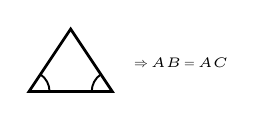
\begin{tikzpicture}[scale=0.48, every node/.style={font=\tiny, text=black}]
      \coordinate (b) at (0,0); \coordinate (c) at (2.2,0); \coordinate (a) at (1.1,1.65);
      \draw[black, line width=1.0pt] (b)--(a)--(c)--cycle;
      \pic[draw=black, line width=0.7pt, angle radius=2.6mm]{angle=c--b--a};
      \pic[draw=black, line width=0.7pt, angle radius=2.6mm]{angle=a--c--b};
      \node[right=3pt] at (2.3,0.75) {$\Rightarrow AB=AC$};
    \end{tikzpicture}} \\ \hline

    \cnum{3} &
    \textbf{បន្ទាត់រួម ៤-ក្នុង-១ ចេញពីកំពូល} &
    ចេញពីកំពូល $A$ ($AB=AC$): មេដ្យាទ័រ $\equiv$ មេដ្យាន $\equiv$ កម្ពស់ $\equiv$ ពុះមុំកំពូល~។ &
    \raisebox{-0.35\height}{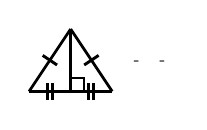
\begin{tikzpicture}[scale=0.48, every node/.style={font=\tiny, text=black}]
      \coordinate (b) at (0,0); \coordinate (c) at (2.2,0); \coordinate (i) at (1.1,0); \coordinate (a) at (1.1,1.65);
      \draw[black, line width=1.0pt, tk1] (a)--(b); \draw[black, line width=1.0pt, tk1] (a)--(c);
      \draw[black, line width=1.0pt, tk2] (b)--(i); \draw[black, line width=1.0pt, tk2] (i)--(c);
      \draw[black, line width=1.0pt] (a)--(i);
      \pic[draw=black, line width=0.7pt, angle radius=1.7mm]{right angle=c--i--a};
      \node[right=2pt] at (2.25,0.75) {៤-ក្នុង-១};
    \end{tikzpicture}} \\ \hline

    \cnum{4} &
    \textbf{ទ្រឹស្ដីបទមេដ្យាទ័រ \& ប្រសព្វ $O$} &
    $M\in\Delta_{AB} \Leftrightarrow MA=MB$; ប្រសព្វមេដ្យាទ័រ $O$ ($OA=OB=OC$)~។ &
    \raisebox{-0.35\height}{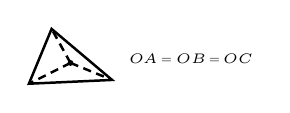
\begin{tikzpicture}[scale=0.48, every node/.style={font=\tiny, text=black}]
      \coordinate (o) at (1.1,0.65); \coordinate (a) at (0.6,1.55); \coordinate (b) at (0,0.1); \coordinate (c) at (2.2,0.2);
      \draw[black, line width=0.9pt] (a)--(b)--(c)--cycle;
      \draw[black, densely dashed, line width=0.9pt] (o)--(a) (o)--(b) (o)--(c);
      \fill[black] (o) circle (2.2pt);
      \node[right=2pt] at (2.25,0.75) {$OA=OB=OC$};
    \end{tikzpicture}} \\ \hline

    \cnum{5} &
    \textbf{លក្ខខណ្ឌត្រីកោណប៉ុនគ្នា និងផលបូកមុំ $180^\circ$} &
    \textbf{ម.ជ.ម / ជ.ម.ជ / ជ.ជ.ជ / អ.ជ} (ហាម \en{SSA}!) និង $\ang{A}+\ang{B}+\ang{C}=180^\circ$~។ &
    \raisebox{-0.35\height}{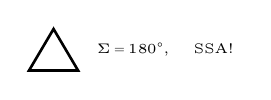
\begin{tikzpicture}[scale=0.48, every node/.style={font=\tiny, text=black}]
      \draw[black, line width=0.95pt] (0,0)--(1.3,0)--(0.65,1.1)--cycle;
      \node[right=2pt] at (1.4,0.55) {$\Sigma=180^\circ$, ហាម \en{SSA}!};
    \end{tikzpicture}} \\ \hline
  \end{tabular}

  \vspace{6pt}

  % --- ផ្នែកទី ៣៖ ប្រៀបធៀប I vs O & ទីតាំង O តាមមុំត្រីកោណ ---
  \noindent
  \begin{minipage}[t]{8.85cm}
    \begin{tcolorbox}[
      enhanced, sharp corners, colback=white, colframe=black,
      boxrule=1.05pt, boxsep=1pt, equal height group=posterBotISO,
      top=5pt, bottom=5pt, left=5pt, right=5pt,
      title={\textbf{ប្រៀបធៀប៖ ប្រសព្វពុះមុំ $I$ \en{vs} ប្រសព្វមេដ្យាទ័រ $O$}},
      colbacktitle=headgray, coltitle=black, fonttitle=\fontsize{8.2pt}{11pt}\selectfont
    ]
      \centering
      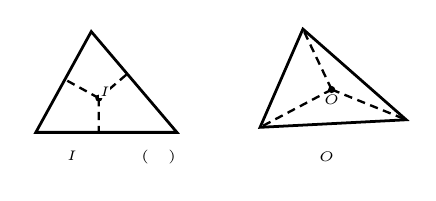
\begin{tikzpicture}[scale=0.64, every node/.style={font=\tiny, text=black}]
        % Left: Incenter I (perpendiculars to 3 sides, always inside)
        \begin{scope}[shift={(0,0)}]
          \coordinate (A) at (1.1,2.0); \coordinate (B) at (0,0); \coordinate (C) at (2.8,0);
          \coordinate (I) at (1.25,0.68);
          \draw[black, line width=1.0pt] (A)--(B)--(C)--cycle;
          \draw[black, densely dashed, line width=0.85pt] (I)--(1.25,0);
          \draw[black, densely dashed, line width=0.85pt] (I)--($(A)!(I)!(B)$);
          \draw[black, densely dashed, line width=0.85pt] (I)--($(A)!(I)!(C)$);
          \fill[black] (I) circle (2.0pt);
          \node[above right=0pt, fill=white, inner sep=0.3pt] at (I) {$I$};
          \node at (1.4,-0.48) {\textbf{ពុះមុំ $I$៖} កែង \textbf{ជ្រុង ៣} (ក្នុង)};
        \end{scope}
        % Right: Circumcenter O (radii to 3 vertices)
        \begin{scope}[shift={(4.45,0)}]
          \coordinate (A) at (0.85,2.05); \coordinate (B) at (0,0.1); \coordinate (C) at (2.9,0.25);
          \coordinate (O) at (1.42,0.85);
          \draw[black, line width=1.0pt] (A)--(B)--(C)--cycle;
          \draw[black, densely dashed, line width=0.85pt] (O)--(A) (O)--(B) (O)--(C);
          \fill[black] (O) circle (2.0pt);
          \node[below=1.5pt, fill=white, inner sep=0.3pt] at (O) {$O$};
          \node at (1.45,-0.48) {\textbf{មេដ្យាទ័រ $O$៖} ទៅ \textbf{កំពូល ៣}};
        \end{scope}
      \end{tikzpicture}
      \par\vspace{3pt}\fontsize{7.7pt}{10.8pt}\selectfont
      $\bullet$ \textbf{ពុះមុំ $I$៖} ស្មើចម្ងាយកែងទៅ\textbf{ជ្រុង ៣} (ស្ថិតនៅ\textbf{ក្នុង}ត្រីកោណជានិច្ច)~។\\
      $\bullet$ \textbf{មេដ្យាទ័រ $O$៖} ស្មើចម្ងាយទៅ\textbf{កំពូល ៣} ($OA=OB=OC$)~។
    \end{tcolorbox}
  \end{minipage}\hfill
  \begin{minipage}[t]{8.85cm}
    \begin{tcolorbox}[
      enhanced, sharp corners, colback=white, colframe=black,
      boxrule=1.05pt, boxsep=1pt, equal height group=posterBotISO,
      top=5pt, bottom=5pt, left=5pt, right=5pt,
      title={\textbf{ទីតាំង $O$ តាមប្រភេទមុំ \en{\&} ប្រយ័ត្នអន្ទាក់ទំ.១៥៧}},
      colbacktitle=midgray, coltitle=black, fonttitle=\fontsize{8.2pt}{11pt}\selectfont
    ]
      \centering
      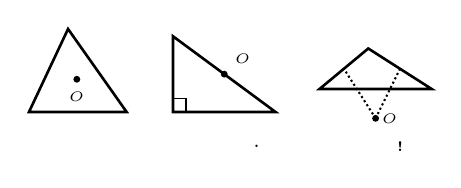
\begin{tikzpicture}[scale=0.62, every node/.style={font=\tiny, text=black}]
        % 1. Acute -> inside
        \begin{scope}[shift={(0,0)}]
          \draw[black, line width=0.95pt] (0,0.15)--(2.0,0.15)--(0.8,1.85)--cycle;
          \fill[black] (0.98,0.82) circle (2.0pt) node[below=1pt] {$O$};
          \node at (1.0,-0.55) {មុំស្រួច៖ \textbf{ក្នុង}};
        \end{scope}
        % 2. Right -> midpoint of hypotenuse
        \begin{scope}[shift={(2.95,0)}]
          \coordinate (r1) at (0,0.15); \coordinate (r2) at (2.1,0.15); \coordinate (r3) at (0,1.70);
          \draw[black, line width=0.95pt] (r1)--(r2)--(r3)--cycle;
          \pic[draw=black, line width=0.65pt, angle radius=1.7mm]{right angle=r2--r1--r3};
          \fill[black] (1.05,0.925) circle (2.0pt) node[above right=0.5pt] {$O$};
          \node at (1.05,-0.55) {មុំកែង៖ \textbf{លើអ៊ីប៉ូ.}};
        \end{scope}
        % 3. Obtuse -> outside (well separated above label at y=-0.55!)
        \begin{scope}[shift={(5.95,0)}]
          \draw[black, line width=0.95pt] (0,0.62)--(1.0,1.45)--(2.3,0.62)--cycle;
          \fill[black] (1.15,0.02) circle (2.0pt) node[right=2pt, fill=white, inner sep=0.3pt] {$O$};
          \draw[black, densely dotted, line width=0.75pt] (1.15,0.02)--(0.5,1.035) (1.15,0.02)--(1.65,1.035);
          \node at (1.15,-0.55) {មុំទាល៖ \textbf{ក្រៅ!}};
        \end{scope}
      \end{tikzpicture}
      \par\vspace{3pt}\fontsize{7.7pt}{10.8pt}\selectfont
      $\bullet$ ត្រីកោណសាមញ្ញ៖ មេដ្យាទ័រ $ON$ \textbf{មិនកាត់}កំពូល $B$ ទេ (\textbf{មេដ្យាទ័រ $\neq$ មេដ្យាន})!
    \end{tcolorbox}
  \end{minipage}
\end{tcolorbox}

\clearpage

% ============================================================================
% ទំព័រទី ៥៖ កាតវិនិច្ឆ័យរហ័ស ៦០–៩០ វិនាទី "កាត A–D" & ចម្លើយគ្រូ — E5 Evaluate
% ============================================================================
\pagebanner{សម្ភារៈទី ៥៖ កាតវិនិច្ឆ័យរហ័ស «កាត \enbf{A--D}» \enbf{(60--90} វិនាទី\enbf{) \&} ចម្លើយគ្រូ}{ទំព័រ ៥/៦ \en{-- E5 Evaluate}}

{\fontsize{8.5pt}{12pt}\selectfont
\textbf{វិធីលេងក្នុងថ្នាក់៖} គ្រូលើកកាតម្ដងមួយ $\rightarrow$ សិស្សផ្ទៀងលក្ខខណ្ឌកំពូល/ប្រភេទមុំ/ចម្ងាយ $I$ \en{vs} $O$ $\rightarrow$ លើក \textbf{មេដៃឡើង (ពិត \ding{51})} ឬ \textbf{ខ្វែងដៃ (ខុស/អន្ទាក់ \ding{55})} + ម្រាម \en{1--3}។}

\vspace{4pt}

% --- ជួរទី ១៖ កាត A & កាត B ---
\noindent
\begin{tcolorbox}[
  enhanced, sharp corners, colback=white, colframe=white,
  borderline={1.0pt}{0pt}{black, dashed},
  width=9.25cm, equal height group=isofoilrow1, nobeforeafter,
  boxsep=1pt, top=5pt, bottom=5pt, left=6pt, right=6pt
]
  \noindent\colorbox{black}{\textcolor{white}{\Large\textbf{\en{ A }}}}\hspace{0.25cm}{\fontsize{9.0pt}{12.2pt}\selectfont\textbf{កាត \en{A} ៖ សមបាទ \en{\&} បន្ទាត់ ៤-ក្នុង-១ ពីកំពូល $A$}}\par\vspace{2pt}
  \begin{center}
  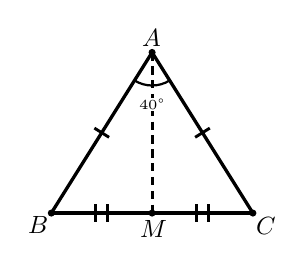
\begin{tikzpicture}[scale=0.80, every node/.style={font=\small, text=black}]
    \coordinate (B) at (0, 0);
    \coordinate (C) at (3.20, 0);
    \coordinate (M) at (1.60, 0);
    \coordinate (A) at (1.60, 2.55);
    \draw[black, line width=1.2pt, tk1] (A) -- (B);
    \draw[black, line width=1.2pt, tk1] (A) -- (C);
    \draw[black, line width=1.2pt, tk2] (B) -- (M);
    \draw[black, line width=1.2pt, tk2] (M) -- (C);
    \draw[black, densely dashed, line width=1.05pt] (A) -- (M);
    \pic[draw=black, line width=0.8pt, angle radius=4.2mm]{angle=B--A--C};
    \node[fill=white, inner sep=0.4pt, font=\tiny] at (1.60, 1.72) {$40^\circ$};
    \fill[black] (A) circle (1.6pt) node[above=1.5pt, fill=white, inner sep=0.4pt] {$A$};
    \fill[black] (B) circle (1.6pt) node[below left=1pt, fill=white, inner sep=0.4pt] {$B$};
    \fill[black] (C) circle (1.6pt) node[below right=1pt, fill=white, inner sep=0.4pt] {$C$};
    \fill[black] (M) circle (1.6pt) node[below=2pt, fill=white, inner sep=0.4pt] {$M$};
  \end{tikzpicture}
  \end{center}
  {\centering\fontsize{7.9pt}{10.8pt}\selectfont $AB=AC$, $\ang{A}=40^\circ$, និង $BM=MC$~។ គេទាញថា $AM\perp BC$, $\ang{BAM}=20^\circ$, $\ang{B}=\ang{C}=70^\circ$~។\par}
  \vfill
  \begin{tcolorbox}[enhanced, sharp corners, colback=panelgray, colframe=black, boxrule=0.8pt, boxsep=1pt, top=4pt, bottom=4pt, left=5pt, right=5pt]
    \centering\fontsize{9.0pt}{12.5pt}\selectfont
    \textbf{សំណួរ៖} តើការសន្និដ្ឋាននេះត្រឹមត្រូវឬទេ?\\[2pt]
    \chkbox\ មេដៃឡើង (\ding{51} ពិត) \hspace{0.4cm} \chkbox\ ខ្វែងដៃ (\ding{55} ខុស)
  \end{tcolorbox}
\end{tcolorbox}%
\hfill
\begin{tcolorbox}[
  enhanced, sharp corners, colback=white, colframe=white,
  borderline={1.0pt}{0pt}{black, dashed},
  width=9.25cm, equal height group=isofoilrow1, nobeforeafter,
  boxsep=1pt, top=5pt, bottom=5pt, left=6pt, right=6pt
]
  \noindent\colorbox{black}{\textcolor{white}{\Large\textbf{\en{ B }}}}\hspace{0.25cm}{\fontsize{9.0pt}{12.2pt}\selectfont\textbf{កាត \en{B} ៖ អន្ទាក់កំពូលខុស ($DE=DF=6, EF=4$)}}\par\vspace{2pt}
  \begin{center}
  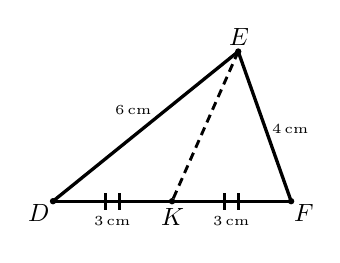
\begin{tikzpicture}[scale=0.72, every node/.style={font=\small, text=black}]
    \coordinate (D) at (0, 0);
    \coordinate (F) at (4.20, 0);
    \coordinate (K) at (2.10, 0);
    \coordinate (E) at (3.2667, 2.6400);
    \draw[black, line width=1.2pt] (D) -- (E) -- (F);
    \draw[black, line width=1.2pt, tk2] (D) -- (K);
    \draw[black, line width=1.2pt, tk2] (K) -- (F);
    \draw[black, densely dashed, line width=1.05pt] (E) -- (K);
    \fill[black] (D) circle (1.6pt) node[below left=1pt, fill=white, inner sep=0.4pt] {$D$};
    \fill[black] (F) circle (1.6pt) node[below right=1pt, fill=white, inner sep=0.4pt] {$F$};
    \fill[black] (K) circle (1.6pt) node[below=2pt, fill=white, inner sep=0.4pt] {$K$};
    \fill[black] (E) circle (1.6pt) node[above=1.5pt, fill=white, inner sep=0.4pt] {$E$};
    \node[above left=1pt, fill=white, inner sep=0.4pt, font=\tiny] at ($(D)!0.55!(E)$) {$6\unit{cm}$};
    \node[right=2pt, fill=white, inner sep=0.4pt, font=\tiny] at ($(E)!0.52!(F)$) {$4\unit{cm}$};
    \node[below=1.5pt, font=\tiny] at (1.05, -0.02) {$3\unit{cm}$};
    \node[below=1.5pt, font=\tiny] at (3.15, -0.02) {$3\unit{cm}$};
  \end{tikzpicture}
  \end{center}
  {\centering\fontsize{7.9pt}{10.8pt}\selectfont $DE=DF=6\unit{cm}$, $EF=4\unit{cm}$ និងមេដ្យាន $EK$ ចេញពី $E$ ទៅកណ្ដាល $K$ នៃ $DF$ ($DK=KF=3\unit{cm}$)~។\par}
  \vfill
  \begin{tcolorbox}[enhanced, sharp corners, colback=panelgray, colframe=black, boxrule=0.8pt, boxsep=1pt, top=4pt, bottom=4pt, left=5pt, right=5pt]
    \centering\fontsize{9.0pt}{12.5pt}\selectfont
    \textbf{សំណួរ៖} គេអះអាងថា $EK \perp DF$ ត្រឹមត្រូវឬទេ?\\[2pt]
    \chkbox\ មេដៃឡើង (\ding{51} ពិត) \hspace{0.4cm} \chkbox\ ខ្វែងដៃ (\ding{55} ខុស)
  \end{tcolorbox}
\end{tcolorbox}

\vspace{6pt}

% --- ជួរទី ២៖ កាត C & កាត D ---
\noindent
\begin{tcolorbox}[
  enhanced, sharp corners, colback=white, colframe=white,
  borderline={1.0pt}{0pt}{black, dashed},
  width=9.25cm, equal height group=isofoilrow2, nobeforeafter,
  boxsep=1pt, top=5pt, bottom=5pt, left=6pt, right=6pt
]
  \noindent\colorbox{black}{\textcolor{white}{\Large\textbf{\en{ C }}}}\hspace{0.25cm}{\fontsize{9.0pt}{12.2pt}\selectfont\textbf{កាត \en{C} ៖ អន្ទាក់ច្រឡំប្រសព្វពុះមុំ $I$ \en{vs} $O$}}\par\vspace{2pt}
  \begin{center}
  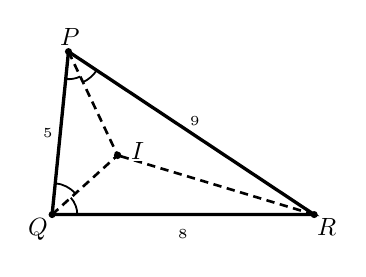
\begin{tikzpicture}[scale=0.80, every node/.style={font=\small, text=black}]
    % Scalene 5, 8, 9 -> P=(0.26, 2.587), Q=(0,0), R=(4.16,0), Incenter I=(1.040, 0.941)
    \coordinate (P) at (0.260, 2.587);
    \coordinate (Q) at (0.000, 0.000);
    \coordinate (R) at (4.160, 0.000);
    \coordinate (I) at (1.040, 0.941);
    \draw[black, line width=1.2pt] (P) -- (Q) -- (R) -- cycle;
    \draw[black, densely dashed, line width=0.95pt] (P) -- (I) (Q) -- (I) (R) -- (I);
    \pic[draw=black, line width=0.65pt, angle radius=3.5mm]{angle=Q--P--I};
    \pic[draw=black, line width=0.65pt, angle radius=4.3mm]{angle=I--P--R};
    \pic[draw=black, line width=0.65pt, angle radius=3.2mm]{angle=R--Q--I};
    \pic[draw=black, line width=0.65pt, angle radius=4.0mm]{angle=I--Q--P};
    \fill[black] (P) circle (1.6pt) node[above=1.5pt, fill=white, inner sep=0.4pt] {$P$};
    \fill[black] (Q) circle (1.6pt) node[below left=1pt, fill=white, inner sep=0.4pt] {$Q$};
    \fill[black] (R) circle (1.6pt) node[below right=1pt, fill=white, inner sep=0.4pt] {$R$};
    \fill[black] (I) circle (1.7pt);
    \node[fill=white, inner sep=0.4pt] at ($(I)+(12:0.32)$) {$I$};
    \node[left=2pt, fill=white, inner sep=0.4pt, font=\tiny] at ($(P)!0.50!(Q)$) {$5$};
    \node[below=1.5pt, font=\tiny] at (2.08, -0.02) {$8$};
    \node[above right=1pt, fill=white, inner sep=0.4pt, font=\tiny] at ($(P)!0.48!(R)$) {$9$};
  \end{tikzpicture}
  \end{center}
  {\centering\fontsize{7.9pt}{10.8pt}\selectfont $\tri{PQR}$ ជ្រុង $5, 8, 9$ មានកន្លះបន្ទាត់ពុះមុំក្នុងប្រសព្វត្រង់ $I$~។ គេអះអាងថា $IP=IQ=IR$~។\par}
  \vfill
  \begin{tcolorbox}[enhanced, sharp corners, colback=panelgray, colframe=black, boxrule=0.8pt, boxsep=1pt, top=4pt, bottom=4pt, left=5pt, right=5pt]
    \centering\fontsize{9.0pt}{12.5pt}\selectfont
    \textbf{សំណួរ៖} តើ $IP=IQ=IR$ ត្រឹមត្រូវឬទេ?\\[2pt]
    \chkbox\ មេដៃឡើង (\ding{51} ពិត) \hspace{0.4cm} \chkbox\ ខ្វែងដៃ (\ding{55} ខុស)
  \end{tcolorbox}
\end{tcolorbox}%
\hfill
\begin{tcolorbox}[
  enhanced, sharp corners, colback=white, colframe=white,
  borderline={1.0pt}{0pt}{black, dashed},
  width=9.25cm, equal height group=isofoilrow2, nobeforeafter,
  boxsep=1pt, top=5pt, bottom=5pt, left=6pt, right=6pt
]
  \noindent\colorbox{black}{\textcolor{white}{\Large\textbf{\en{ D }}}}\hspace{0.25cm}{\fontsize{9.0pt}{12.2pt}\selectfont\textbf{កាត \en{D} ៖ អន្ទាក់ប្រសព្វ $O$ ក្នុងត្រីកោណមុំទាល ($120^\circ$)}}\par\vspace{2pt}
  \begin{center}
  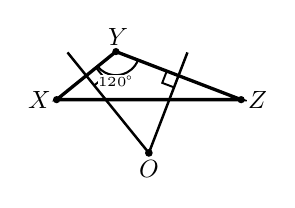
\begin{tikzpicture}[scale=0.82, every node/.style={font=\small, text=black}]
    % Obtuse XYZ: angle Y = 120 deg, O=(1.80, 0.65), R=1.65
    \coordinate (O) at (1.8000, 0.6500);
    \coordinate (X) at (0.3711, 1.4750);
    \coordinate (Y) at (1.2901, 2.2192);
    \coordinate (Z) at (3.2289, 1.4750);
    \coordinate (M1) at ($(X)!0.5!(Y)$);
    \coordinate (M2) at ($(Y)!0.5!(Z)$);
    \draw[black, line width=1.2pt] (X) -- (Y) -- (Z) -- cycle;
    \draw[black, line width=0.9pt] (O) -- ($(O)!1.30!(M1)$);
    \draw[black, line width=0.9pt] (O) -- ($(O)!1.30!(M2)$);
    \pic[draw=black, line width=0.7pt, angle radius=1.6mm]{right angle=O--M1--Y};
    \pic[draw=black, line width=0.7pt, angle radius=1.6mm]{right angle=O--M2--Y};
    \pic[draw=black, line width=0.75pt, angle radius=3.0mm]{angle=X--Y--Z};
    \node[fill=white, inner sep=0.3pt, font=\tiny] at ($(Y)+(-90:0.46)$) {$120^\circ$};
    \fill[black] (X) circle (1.6pt) node[left=2pt, fill=white, inner sep=0.4pt] {$X$};
    \fill[black] (Y) circle (1.6pt) node[above=1.5pt, fill=white, inner sep=0.4pt] {$Y$};
    \fill[black] (Z) circle (1.6pt) node[right=2pt, fill=white, inner sep=0.4pt] {$Z$};
    \fill[black] (O) circle (1.7pt) node[below=2pt, fill=white, inner sep=0.4pt] {$O$};
  \end{tikzpicture}
  \end{center}
  {\centering\fontsize{7.9pt}{10.8pt}\selectfont ក្នុង $\tri{XYZ}$ ($\ang{Y}=120^\circ$) $O$ ជាប្រសព្វមេដ្យាទ័រ។ គេអះអាងថា $O$ ស្ថិតនៅ\textbf{ខាងក្នុង} $\tri{XYZ}$ ជានិច្ច~។\par}
  \vfill
  \begin{tcolorbox}[enhanced, sharp corners, colback=panelgray, colframe=black, boxrule=0.8pt, boxsep=1pt, top=4pt, bottom=4pt, left=5pt, right=5pt]
    \centering\fontsize{9.0pt}{12.5pt}\selectfont
    \textbf{សំណួរ៖} តើ $O$ នៅខាងក្នុង $\tri{XYZ}$ ត្រឹមត្រូវឬទេ?\\[2pt]
    \chkbox\ មេដៃឡើង (\ding{51} ពិត) \hspace{0.4cm} \chkbox\ ខ្វែងដៃ (\ding{55} ខុស)
  \end{tcolorbox}
\end{tcolorbox}

\vspace{6pt}

% --- ខ្សែកាត់ & បន្ទះចម្លើយសម្រាប់គ្រូ ---
\noindent\scissors\ \dotfill\ \textbf{កាត់ទុកសម្រាប់គ្រូ (\en{Teacher Mini Answer \& Remediation Key})} \dotfill\ \scissors

\vspace{4pt}
\begin{tcolorbox}[
  enhanced, sharp corners, colback=panelgray, colframe=black,
  boxrule=1.0pt, boxsep=1pt, top=4pt, bottom=4pt, left=5pt, right=5pt
]
  \fontsize{7.65pt}{10.6pt}\selectfont
  \renewcommand{\arraystretch}{1.10}
  \begin{tabular}{|L{4.25cm}|L{4.25cm}|L{4.25cm}|L{4.25cm}|}
    \hline
    \cellcolor{headgray}\textbf{កាត \en{A} ៖ មេដៃឡើង (\ding{51})} &
    \cellcolor{headgray}\textbf{កាត \en{B} ៖ ខ្វែងដៃ (\ding{55})} &
    \cellcolor{headgray}\textbf{កាត \en{C} ៖ ខ្វែងដៃ (\ding{55})} &
    \cellcolor{headgray}\textbf{កាត \en{D} ៖ ខ្វែងដៃ (\ding{55})} \\ \hline
    \textbf{ពិត!} $AB=AC$ និង $M$ កណ្ដាល $BC$ $\Rightarrow AM$ ជាបន្ទាត់ \textbf{៤-ក្នុង-១} (\cnum{3}) ពីកំពូល $A$: $AM\perp BC$, $\ang{BAM}=20^\circ$, $\ang{B}=\ang{C}=70^\circ$ (\cnum{1}, \cnum{5})។ &
    \textbf{អន្ទាក់កំពូលខុស!} $D$ ទើបជាកំពូល ($DE=DF=6$) មិនមែន $E$ ទេ ($ED\neq EF$)! មេដ្យាន $EK$ ចេញពីកំពូលបាត \textbf{មិនកែង} $DF$ ទេ ($EK\not\perp DF$)។ &
    \textbf{ច្រឡំ $I$ នឹង $O$!} ប្រសព្វពុះមុំ $I$ ស្មើចម្ងាយកែងទៅ\textbf{ជ្រុង ៣} មិនមែនកំពូល $P, Q, R$ ទេ! ប្រសព្វមេដ្យាទ័រ $O$ (\cnum{4}) ទើប $OP=OQ=OR$។ &
    \textbf{អន្ទាក់មុំទាល!} $\ang{Y}=120^\circ > 90^\circ$ $\Rightarrow$ ប្រសព្វមេដ្យាទ័រ $O$ ស្ថិតនៅ\textbf{ខាងក្រៅ} $\tri{XYZ}$ (ឈមមុំទាល $120^\circ$)! \\ \hline
  \end{tabular}
  \par\vspace{2.5pt}
  \textbf{ត្រួតទំនុកចិត្ត (ម្រាម ១\en{--}៣)៖} ១ ម្រាម = សុំដៃគូពន្យល់ \hspace{0.15cm}\en{|}\hspace{0.15cm} ២ ម្រាម = ផ្ទៀងធនាគារ \cnum{1}--\cnum{5} \hspace{0.15cm}\en{|}\hspace{0.15cm} ៣ ម្រាម = ច្បាស់ ១០០\%
\end{tcolorbox}

\clearpage

% ============================================================================
% ទំព័រទី ៦៖ ប័ណ្ណកិច្ចការផ្ទះ ជំហានទី ៥ — ៤ ប័ណ្ណក្នុង ១ ទំព័រ A4 (4-up: HW #2, #8, #11)
% ============================================================================
\pagebanner{សម្ភារៈទី ៦៖ ប័ណ្ណកិច្ចការផ្ទះ ជំហានទី ៥ \enbf{--} ៤ ប័ណ្ណក្នុង ១ ទំព័រ \enbf{A4}}{ទំព័រ ៦/៦ \en{--} ជំហានទី ៥ (កាត់ ៤ ប័ណ្ណ \scissors)}

% ម៉ាក្រូប័ណ្ណកិច្ចការផ្ទះ ៤-up (ផ្ទៀង ១០០% នឹងលំហាត់ទី ២ ទំ.១៦៤ និងទី ៨, ទី ១១ ទំ.១៦៥)
\newcommand{\hwslipFourISO}[1]{%
\begin{tcolorbox}[
  enhanced, sharp corners, colback=white, colframe=white,
  borderline={0.95pt}{0pt}{black, dashed},
  width=9.25cm, equal height group=hwquadISO, nobeforeafter,
  boxsep=1pt, top=2.5pt, bottom=2.5pt, left=4pt, right=4pt
]
  \begin{tcolorbox}[
    enhanced, sharp corners, colback=headgray, colframe=black,
    boxrule=0.7pt, boxsep=1pt, top=1.5pt, bottom=1.5pt, left=4pt, right=4pt, after skip=2pt
  ]
    \fontsize{7.1pt}{9.6pt}\selectfont
    \textbf{\scissors\ កិច្ចការផ្ទះ (#1) \en{|} ២.២ សមបាទ \& ប្រសព្វ} \hfill \textbf{ពុធ ០២/១២/២៦}\\[1pt]
    ឈ្មោះ៖ $\underline{\hspace{4.0cm}}$ \hspace{0.2cm} ថ្នាក់៖ $\underline{\hspace{1.0cm}}$
  \end{tcolorbox}

  % --- លំហាត់ទី ២ (សៀវភៅទំព័រ ១៦៤) ---
  \noindent
  \begin{minipage}[c]{5.25cm}
    \fontsize{6.8pt}{9.3pt}\selectfont
    \textbf{លំហាត់ទី ២ (ទំ.១៦៤)៖} គេឱ្យ $PQ=PR$ និង $\ang{PST}=\ang{PTS}$~។ ប្រៀបធៀប $\tri{PQS}$ និង $\tri{PRT}$~។\\
    {\fontsize{6.3pt}{8.7pt}\selectfont\textit{អន្ទាក់ \en{SSA}!} ហាមប្រើ \en{SSA}! ប្រើ $\ang{Q}=\ang{R}$ (\cnum{1}) \en{+} $\ang{PSQ}=\ang{PTR}$ \en{+} ផលបូក $180^\circ \Rightarrow \ang{QPS}=\ang{RPT}$ (\textbf{ម.ជ.ម} ឬ \textbf{ជ.ម.ជ})!}
  \end{minipage}\hfill
  \begin{minipage}[c]{3.35cm}
    \centering
    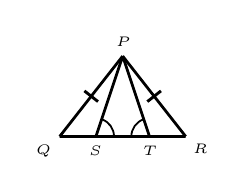
\begin{tikzpicture}[scale=0.40, every node/.style={font=\tiny, text=black}]
      \coordinate (Q) at (0,0); \coordinate (S) at (1.15,0); \coordinate (T) at (2.85,0); \coordinate (R) at (4.0,0);
      \coordinate (P) at (2.0,2.55);
      \draw[black, line width=1.0pt] (Q)--(R) (P)--(S) (P)--(T);
      \draw[black, line width=1.0pt, tk1] (P)--(Q);
      \draw[black, line width=1.0pt, tk1] (P)--(R);
      \pic[draw=black, line width=0.65pt, angle radius=2.3mm]{angle=T--S--P};
      \pic[draw=black, line width=0.65pt, angle radius=2.3mm]{angle=P--T--S};
      \node[above=0pt] at (P) {$P$}; \node[below left=-1pt] at (Q) {$Q$};
      \node[below=0pt] at (S) {$S$}; \node[below=0pt] at (T) {$T$}; \node[below right=-1pt] at (R) {$R$};
    \end{tikzpicture}
  \end{minipage}

  \vspace{2pt}\hrule height 0.45pt\vspace{2pt}

  % --- លំហាត់ទី ៨ (សៀវភៅទំព័រ ១៦៥) ---
  \noindent
  \begin{minipage}[c]{5.25cm}
    \fontsize{6.8pt}{9.3pt}\selectfont
    \textbf{លំហាត់ទី ៨ (ទំ.១៦៥)៖} $\tri{ABC}$ សមបាទកំពូល $A$, $M, N$ ជាចំណុចកណ្ដាល $AB, AC$, $P=BN\cap CM$~។ បង្ហាញថា $\tri{PBC}$ សមបាទ~។\\
    {\fontsize{6.3pt}{8.7pt}\selectfont\textit{តម្រុយ៖} គូសសញ្ញា $BM=CN$, $\ang{MBC}=\ang{NCB}$ \en{+} \en{[tracing]} $\tri{MBC}\cg\tri{NCB}$ (\textbf{ជ.ម.ជ}) $\Rightarrow \ang{PBC}=\ang{PCB} \Rightarrow$ \cnum{2}!}
  \end{minipage}\hfill
  \begin{minipage}[c]{3.35cm}
    \centering
    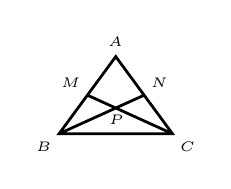
\begin{tikzpicture}[scale=0.40, every node/.style={font=\tiny, text=black}]
      \coordinate (B) at (0,0); \coordinate (C) at (3.6,0); \coordinate (A) at (1.8,2.45);
      \coordinate (M) at ($(A)!0.5!(B)$); \coordinate (N) at ($(A)!0.5!(C)$);
      \coordinate (P) at (1.8, 0.8167);
      \draw[black, line width=1.0pt] (A)--(B)--(C)--cycle (B)--(N) (C)--(M);
      \node[above=0pt] at (A) {$A$}; \node[below left=-1pt] at (B) {$B$}; \node[below right=-1pt] at (C) {$C$};
      \node[above left=-1pt] at (M) {$M$}; \node[above right=-1pt] at (N) {$N$};
      \node[below=2pt, fill=white, inner sep=0.3pt] at (P) {$P$};
    \end{tikzpicture}
  \end{minipage}

  \vspace{2pt}\hrule height 0.45pt\vspace{2pt}

  % --- លំហាត់ទី ១១ (សៀវភៅទំព័រ ១៦៥) ---
  \noindent
  \begin{minipage}[c]{5.25cm}
    \fontsize{6.8pt}{9.3pt}\selectfont
    \textbf{លំហាត់ទី១១ (ទំ.១៦៥)៖} \mbox{$HO\perp OB$}, \mbox{$DB\perp OB$}, $OP=BE, HO=DB$~។ បង្ហាញថា \textbf{(ក)} $\tri{HOE}\cg\tri{DBP}$ \textbf{(ខ)} $\tri{FPE}$ សមបាទ~។\\
    {\fontsize{6.3pt}{8.7pt}\selectfont\textit{តម្រុយ៖} (ក) បូក $OE=OP+PE=BE+PE=BP \Rightarrow$ \textbf{ជ.ម.ជ}; (ខ) $\ang{FEP}=\ang{FPE} \Rightarrow$ \cnum{2} $FP=FE$!}
  \end{minipage}\hfill
  \begin{minipage}[c]{3.35cm}
    \centering
    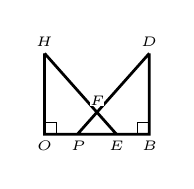
\begin{tikzpicture}[scale=0.38, every node/.style={font=\tiny, text=black}]
      \coordinate (O) at (0,0); \coordinate (P) at (1.1,0); \coordinate (E) at (2.4,0); \coordinate (B) at (3.5,0);
      \coordinate (H) at (0,2.7); \coordinate (D) at (3.5,2.7);
      \coordinate (F) at (1.75, 0.731);
      \draw[black, line width=1.0pt] (H)--(O)--(B)--(D) (H)--(E) (D)--(P);
      \pic[draw=black, line width=0.6pt, angle radius=1.5mm]{right angle=P--O--H};
      \pic[draw=black, line width=0.6pt, angle radius=1.5mm]{right angle=D--B--E};
      \node[above=-1pt] at (H) {$H$}; \node[above=-1pt] at (D) {$D$};
      \node[below=-1pt] at (O) {$O$}; \node[below=-1pt] at (P) {$P$};
      \node[below=-1pt] at (E) {$E$}; \node[below=-1pt] at (B) {$B$};
      \node[above=2pt, fill=white, inner sep=0.3pt] at (F) {$F$};
    \end{tikzpicture}
  \end{minipage}

  \vspace{2pt}
  \begin{tcolorbox}[
    enhanced, sharp corners, colback=panelgray, colframe=black,
    boxrule=0.7pt, boxsep=1pt, top=2pt, bottom=2pt, left=4pt, right=4pt
  ]
    \fontsize{6.55pt}{9.1pt}\selectfont
    \textbf{ផ្ទៀងខ្លួនឯង (\en{Warrant \cnum{1}--\cnum{5}})៖}
    \chkbox\ ជៀសវាងអន្ទាក់ \en{SSA} (លំ.២) \en{|} \chkbox\ គូសសញ្ញាលើរូប (លំ.៨) \en{|} \chkbox\ ដាក់លេខ \cnum{1}--\cnum{5} គ្រប់ជំហាន (២, ៨, ១១)!
  \end{tcolorbox}
\end{tcolorbox}%
}

\noindent
\hwslipFourISO{ប័ណ្ណទី ១}\hfill\hwslipFourISO{ប័ណ្ណទី ២}

\vspace{5.5pt}
\noindent\scissors\ \dotfill\ \textbf{កាត់តាមស្នាមចុចចែកជា ៤ ប័ណ្ណ (\en{Cut Along Dashed Lines})} \dotfill\ \scissors
\vspace{5.5pt}

\noindent
\hwslipFourISO{ប័ណ្ណទី ៣}\hfill\hwslipFourISO{ប័ណ្ណទី ៤}

\end{document}
